% This is "sig-alternate.tex" V2.0 May 2012
% This file should be compiled with V2.5 of "sig-alternate.cls" May 2012
\def\year{2015}
%File: formatting-instruction.tex
\documentclass[letterpaper]{article}
\usepackage{aaai}
\usepackage{tabularx}
\usepackage{times}
\usepackage{helvet}
\usepackage{courier}
\usepackage{epsfig}
\usepackage{epstopdf}
\usepackage{booktabs}
\usepackage{color, colortbl}
\usepackage{amsmath}
\usepackage{tikz}
\usepackage{pdfsync}
\usepackage{multirow}
\usepackage{url}
%\usepackage[none]{hyphenat}
\usetikzlibrary{arrows}

\newtheorem{problem}{Problem}
\newtheorem{definition}{Definition}
\newtheorem{pdef}{Problem Definition}
\newtheorem{theorem}{Theorem}
\newtheorem{example}{Example}
\newtheorem{obser}{{Observation}}
\newtheorem{lemma}{{Lemma}}

\DeclareMathOperator*{\argmin}{arg\,min}
\DeclareMathOperator*{\argmax}{arg\,max}

% insert graph
%\renewcommand\textfraction{}
% emphasize,terms
\newcommand{\term}[1]{{\tt#1}}
\newcommand{\Red}[1]{\textcolor[rgb]{1.00,0.00,0.00}{#1}}
\newcommand{\Blue}[1]{\textcolor[rgb]{0.00,1.00,0.00}{#1}}
\newcommand{\Green}[1]{\textcolor[rgb]{0.00,0.00,1.00}{#1}}
\newcommand{\xch}[1]{\Blue{#1}}
\newcommand{\yh}[1]{\Red{#1}}
\newcommand{\nop}[1]{}
%\newcommand{\isa}[0]{$ \stackrel{  isA  }{\longrightarrow} $ }
\newcommand{\isa}{ isA }
\newcommand{\noisa}[0]{$ \stackrel{ Head }{\dashrightarrow} $ }

\newcommand{\at}[1]{{\small\tt #1}}
\newcommand{\ac}[1]{\emph{#1}}

%\renewcommand{\baselinestretch}{0.98} 


\begin{document}

%\title{Implicit Relation Inferring Using Knowledge Graph}
\title{From Hyperlinks to Semantic Links: A Probabilistic Approach to Explain Hyperlinks in Wikipedia}
%\subtitle{A Probabilistic Approach to Explain Hyperlinks in Wikipedia}

%\numberofauthors{8}

%\author{
% 1st. author
%\alignauthor
%Ben Trovato\titlenote{Dr.~Trovato insisted his name be first.}\\
%       \affaddr{Institute for Clarity in Documentation}\\
%       \affaddr{1932 Wallamaloo Lane}\\
%       \affaddr{Wallamaloo, New Zealand}\\
%       \email{trovato@corporation.com}


\maketitle
\begin{abstract}

In this paper, we present Entity Relation Finder ($ERF$): a framework of semantifying 
the relationship between a Wikipedia page and another page hyperlinked from the page.
This is an easy task if there already exists a triple in the knowledge base explaining the relationship
between the given entity pair.
However, this is only the 1.5\% of the cases, and for the rest, we need to infer a triple between the entity pair.
We propose to conceptualize entity pair into proper concept pairs, as intermediate random variables.
Though entity conceptualization has been studied, this has new challenges of jointly optimizing for both entities and aggregating diluted observations into the head concepts defining the relationship.
Meanwhile, there is an opportunity of leveraging existing triples and concept probabilities of web-scale taxonomy, for such probabilistic reasoning.
We validate our proposed framework using real-life entity pairs and Probase taxonomy.

\end{abstract}

%\keywords{ACM proceedings, \LaTeX, text tagging}
\vspace{-2mm}
\section{Introduction}


Semantifying web documents is a huge task. Recently, more and more hyperlinked documents emerge. There are almost semi-structured information everywhere, but unfortunately the links lacks an explanation of why they are connected, and why human may consider them related[]. The types of hyperlink are article to article, article to knowledge base(or encyclopedia-like databases). Each link has two ends the original one(the web page/ entity page contains it) and the oriented one(the web page/ entity page it points to), and each end has 2 possible types, an anchor url or an anchor entity. Hence, in all there are 4 possible combinations, which consists the 4 type of links.
An anchor entity can be named entities such as movies, products, people names, locations etc. In this case we explain the relation between the entity and the original article. As for an anchor url, an automatic target entity extraction process[2011] can be performed, and then it become another semantifying problem between entities problem.

In this paper we focus on the problem of semantifying the first type of hyperlinks since other kinds of links can finally be deduced to this problem.

We argue that the context of an entity in an article is informative[] and deserve a higher occurrence[] and can produce fresh and latest relation of an entity, which can be useful in updating the KB[reverb]. In our approach the relations is not necessarily to be exist, however the cluster of the relation[relation clustering] it belongs to should be conceptually right. For instance, the relationship {\tt artist of} will be correct in the tuple of {\tt(Leonardo Da Vinci, artist of, Mona Lisa)} [{\tt(Human, artist of, Painting)}] and will be never correct in the tuple of {\tt (Automobile, artist of, Painting)} [e.g.{\tt(BMW i8,artist of, Mona Lisa )}]
With rich context and large knowledge base, we can easily derive the fresh context relations and the concept of each entity, 

On the other hand, we consider the co-occurrence of the 2 entities, based on the assumption of important relationship will be observed in various of documents[]

For these reasons, we purpose a relation explanation method leveraging the concept and co-occurrence of and entity, to explain the relation between the target entity and the related entity, thus semantifying the hyperlink.

\vspace{-2mm}
\section{Related Works}
%improves: incrementally training the entity-concepts so that it can model time varying attributes.(phone,manufacturer,company)--after2007-->(smartphone ,manufacturer,company)




%perform NER~\cite in the document to link the entities.

\subsection{Relation Explanation}


Various of efforts are devoted to relation Explanation.
Blanco et al.~\cite{blanco2010finding} study the problem of finding support sentences to explain the relationship between a named entity and an ad-hoc query.
Fang et al.~\cite{fang2011rex} explain the relation ship between 2 entities by answering a subgraph from the knowledge base.
Voskarides et al.~\cite{voskarideslearning} models the problem of explaining relationship between entities into sentences retrieval problem, ranking the explanation sentence from Wikipedia by how well it describe the relationship.
All these tasks takes the relation between entities as given input from knowledge graph, in this paper, we retrieve the most probable relation for a given entity pair.

~\cite{shahaf2010connecting,luo2007answering} are on graph based approaches and text based approaches~\cite{hasegawa2004discovering}[reverb].
\xch{~\cite{nakashole2013discovering,nakashole2012discovering,konstantinova2014review}}
However, these approached will be limited largely by the incompletion of Knowledge Base, and cannot discover new type of relations.
In our work, we focus on semantic relations of entity by leveraging the concepts of entity. extracted from knowledge bases to link entities with a probability.


\subsection{Information Extraction}

Attribute acquisition methods
Among domain-dependent approaches, we can mention approaches that focus on products. In this domain, attributes have been used to improve product search and recommendation [18, 22], but also to enable data mining [27]

Attribute retrieval provides another granularity in Web
search. This can interest communities that propose a more
focused access to information or communities that envision
aggregating pieces of information such as aggregated search
[19, 15].
Wong et al. [27]
combine tags and textual features in a Conditional Random
Fields model to learn attribute extraction rules, but they
need a seed of relevant documents manually fed.


\subsection{Link entities to Database}

Linking entities to database, especially to Wikipedia, has been widely studied. Entity linking to Wikipedia~\cite{milne2008learning,mihalcea2007wikify,han2011collective} exploit Wikipedia as thesaurus and link web documents to it.
In our work, instead of linking entities to the correspond one in KB, we extract the target entity~\cite{dalvi2011automatic} and explain the semantic relation of the entity towards target entity.


\subsection{Short Text Conceptualization}

\vspace{-2mm}

% !TEX root = main.tex
\section{Problem Model}
\label{sec:framework}
In this section, we formalize our problem, followed by a restatement based on concept based inference.
\vspace{-2mm}
\paragraph{Problem Formalization}
For a given pair of entity, we formalize the problem of explaining the relationship between them as finding the attribute with a probability ranking.
More formally, given an entity pair $ \langle e_1, e_2 \rangle $, we want to find:
\begin{equation}
\argmax_a P(a|\langle e_1,e_2 \rangle),
\end{equation}
where $P(a| \langle e_1, e_2 \rangle )$ is the probability that $a$ is an attribute between two entities. Similarly, we later use $P(a| \langle c_{1},c_{2} \rangle )$ to denote the {\it typicality} of attribute $a$ given the concept pair.

For example, for entity pair \at{<Bill Gates, Microsoft>}, \at{FounderOf, BoardOf} are among the most probable relations.
However relation like \at{KeyPeopleOf} is not that typical. 

%We give notations used in this paper in Table~\ref{tab:notation}.
\vspace{-2mm}
\paragraph{Concept-based Inference}
Thus our problem is reduced to the estimation of $P(a| \langle e_1, e_2 \rangle )$.
The direct estimation is difficult since no such samples are available.
We resort to the concepts of entities to bridge the inference from entity pair to their attribute.
The rationality comes from the observation that {\it it is the concept determines the relationship between entities}. For example, \at{<Washington, USA>} can be best explained by \at{CapitalOf} attribute, which essentially is determined by the concept pair \at{<Capital City, Country>}.
In other words, a relationship can be considered as generated by corresponding concept pairs.
The entity pairs that belong to the same concept pairs share the same relationship explanation.
Continue the previous example, \at{<Beijing, China>} is clearly another example of entity pairs belonging to \at{<Capital, Country>} that can be explained by the \at{CapitalOf} attribute.

Using concept pairs as intermediate random variables, our problem can be restated as:
\begin{equation}
\label{eq:target}
\small
\argmax_a \sum_{c_i\in C_1 , c_j \in C_2 }P(a|\langle c_{i},c_{j}\rangle)\times P(\langle c_{i},c_{j}\rangle|\langle e_{1},e_{2}\rangle),
\end{equation}
where $P(a|\langle c_{1},c_{2}\rangle)$ is the probability that attribute $a$ is relationship between the concept pair
and $P(\langle c_{i},c_{j}\rangle |\langle e_{1},e_{2}\rangle)$ is the probability that $\langle c_1, c_2\rangle$ is the concept pair of $ \langle e_1, e_2 \rangle $.
%\nop{
%For the same concept pair, some attribute is more typical than another one.
%For concept pair \at{<artist, country>}, the attribute \ac{hometown} is more typical than \ac{education}.
%For a given entity pair, some concept pair is better to characterize the concept of the entity pair than others.
%As example,  for \at{<apple, Steve Jobs>},  \at{<company, entrepreneur>} deserves a higher probability than \at{<food, name>}.
%$P( \langle c_{i},c_{j} \rangle | \langle e_{1},e_{2} \rangle )$ can also be considered as the typicality of the concept pair for the given entity pair.
%
%
%Another benefit of concept-level estimation is that it can reduce the computation cost.
%In general, the number of concept pairs is significantly less than that of entity pairs.
%}

\vspace{-2mm}

\section{Joint Conceptualization}
In this section, we present our solution to estimate $ P(\langle c_1,c_2 \rangle | \langle e_1,e_2\rangle) $.
Our basic idea is considering the conceptualization of $e_1$ and $e_2$ jointly instead of independently.
By joint conceptualization, we derive a new optimization objective function.


\paragraph{Estimation of $P(\langle c_1,c_2\rangle | \langle e_1,e_2\rangle)$ }
A straightforward estimation of $P( \langle c_{1},c_{2} \rangle | \langle e_{1},e_{2} \rangle )$ is as Eq.~\ref{eq:naive} when we assume that the choice of concept for $e_1$ is independent of that for $e_2$.
\begin{equation}
\label{eq:naive}
\small
\begin{split}
P(\langle c_{1},c_{2}\rangle |\langle e_{1},e_{2} \rangle) = P(c_1|e_1) P(c_2|e_2)
\end{split}
\end{equation} The rationale is that the typicality of a concept pair can be quantified as the product of the respective typicality of each concept given its corresponding entity.
However, the assumption does not always hold as shown in Example~\ref{exa:jc}. Hence, we need to introduce a factor $\alpha(c_1,c_2)$ into Eq.~\ref{eq:target_expand2_jr} to quantify {\it how likely that the two concepts are the appropriate concepts of the attribute}. Thus, we have the following improved estimation:
\begin{equation}
\label{eq:target_expand2_jr}
\small
\begin{split}
P(\langle c_{1},c_{2}\rangle |\langle e_{1},e_{2} \rangle) = \alpha(c_1,c_2)  P(c_1|e_1)  P(c_2|e_2)
\end{split}
\end{equation}


One simple estimation of $\alpha(c_1,c_2)$ is using the prior probability of $\langle c_1, c_2\rangle$, i.e., $P(\langle c_1,c_2\rangle)$ (see Eq.~\ref{eq:rel_jdp}).
\begin{equation}\label{eq:rel_jdp}
\small
  \alpha(c_1,c_2) = P(\langle c_1, c_2\rangle)
\end{equation}
This is reasonable since the true concept pair for an entity pair in general has a larger probability than
a false concept pair.

Using Bayesian rules, $P(a| \langle c_{1},c_{2} \rangle )$ can be restated by the following equation:
\begin{equation}
\label{eq:target_expand1}
\small
P(a|\langle c_{1},c_{2} \rangle)= \frac{ P(\langle c_{1},c_{2}\rangle|a)P(a) }{ P(\langle c_{1},c_{2}\rangle) }
\end{equation},
where $P(a)$ is probability to observe an entity pair with attribute $a$.
Thus the objective function is reduced to Eq.~\ref{eq:simple_obj} when Eq.~\ref{eq:rel_jdp} holds.
\begin{equation}
\label{eq:simple_obj}
\small
 \argmax_a \sum_{c_i\in C_1, c_j\in C_2} P(\langle c_{i},c_{j}\rangle |a) P(a) P(c_i|e_1) P(c_j|e_2)
\end{equation}




%\nop{
%\subsection{Target Expand}
%Given, Eq~\ref{eq:target}, the estimation of $P(a| \langle e_1,e_2 \rangle )$ boils down to 2 parts:
%\begin{enumerate}
%\item $P(a| \langle c_{1},c_{2} \rangle )$:  the typicality of an attribute for a concept pair.
%\item $P( \langle c_{i},c_{j} \rangle | \langle e_{1},e_{2} \rangle )$:  the typicality of the concept pair for an entity pair.
%\end{enumerate}
%
%Using Bayesian rules, $P(a| \langle c_{1},c_{2} \rangle )$ can be restated in Eq.\ref{eq:target_expand1}:
%\begin{equation}
%\label{eq:target_expand1}
%\begin{split}
%P(a|\langle c_{1},c_{2} \rangle) &= \frac{ P(\langle c_{1},c_{2}\rangle|a)\times P(a) }{ P(\langle c_{1},c_{2}\rangle) }
%%&=\frac{ p((c_{1},c_{2})|a)\times P(a) }{ \sum{P( (c_{1},c_{2})|a^* )\times P(a^*)   } },
%\end{split}
%\end{equation},
%where $P(a)$ is probability to observe an entity pair with attribute $a$.
%}

\paragraph{Solution Framework}
Now we are ready to present our framework. The main framework is illustrated in Figure~\ref{fig:framework}, which consists of two major components: {\it online computation} and {\it offline training}. 
We refer to our system as \ac{Entity Relation Finder ($ERF$)}.
$ERF$ takes an entity pair as input and find its most plausible relation as the result.
As a preprocessing step, we first directly lookup the attribute for the query entity pair from DBpedia.
If DBpedia has SPO triples connecting the entity pair, we direct return the predicate as the answer.
Otherwise, the procedure goes into the online computation component.
The online component calculates $ P(a|  \langle e_1,e_2 \rangle  )$ for each candidate attribute in $A$ (the set of all attributes) by Eq.~\ref{eq:simple_obj} and return the maximal one as the answer attribute. To compute Eq.~\ref{eq:simple_obj}, we need to compute $P(\langle c_1,c_2 \rangle |a)$, $P(a)$, $P(c_1|e_1)$ and $P(c_2|e_2)$. 

In the online part, we compute $P(c_1|e_1)$ and $P(c_2|e_2)$.
One possible solution is materializing them for all possible $\langle e_1,e_2 \rangle$ pair in the offline computing.
Unfortunately, we cannot predict which entity pair would occur as a query so that a materialization often suffers from quadratic complexity, which is unaffordable when we have millions of entities. 
In the offline part, we compute $P(c_1,c_2|a)$ and $P(a)$ by leveraging the SPO triples in DBpedia and isA relationships in $Probase$. 
We elaborate the detail in the next section.

\begin{figure}[!t]
\vspace{-4mm}
\centering
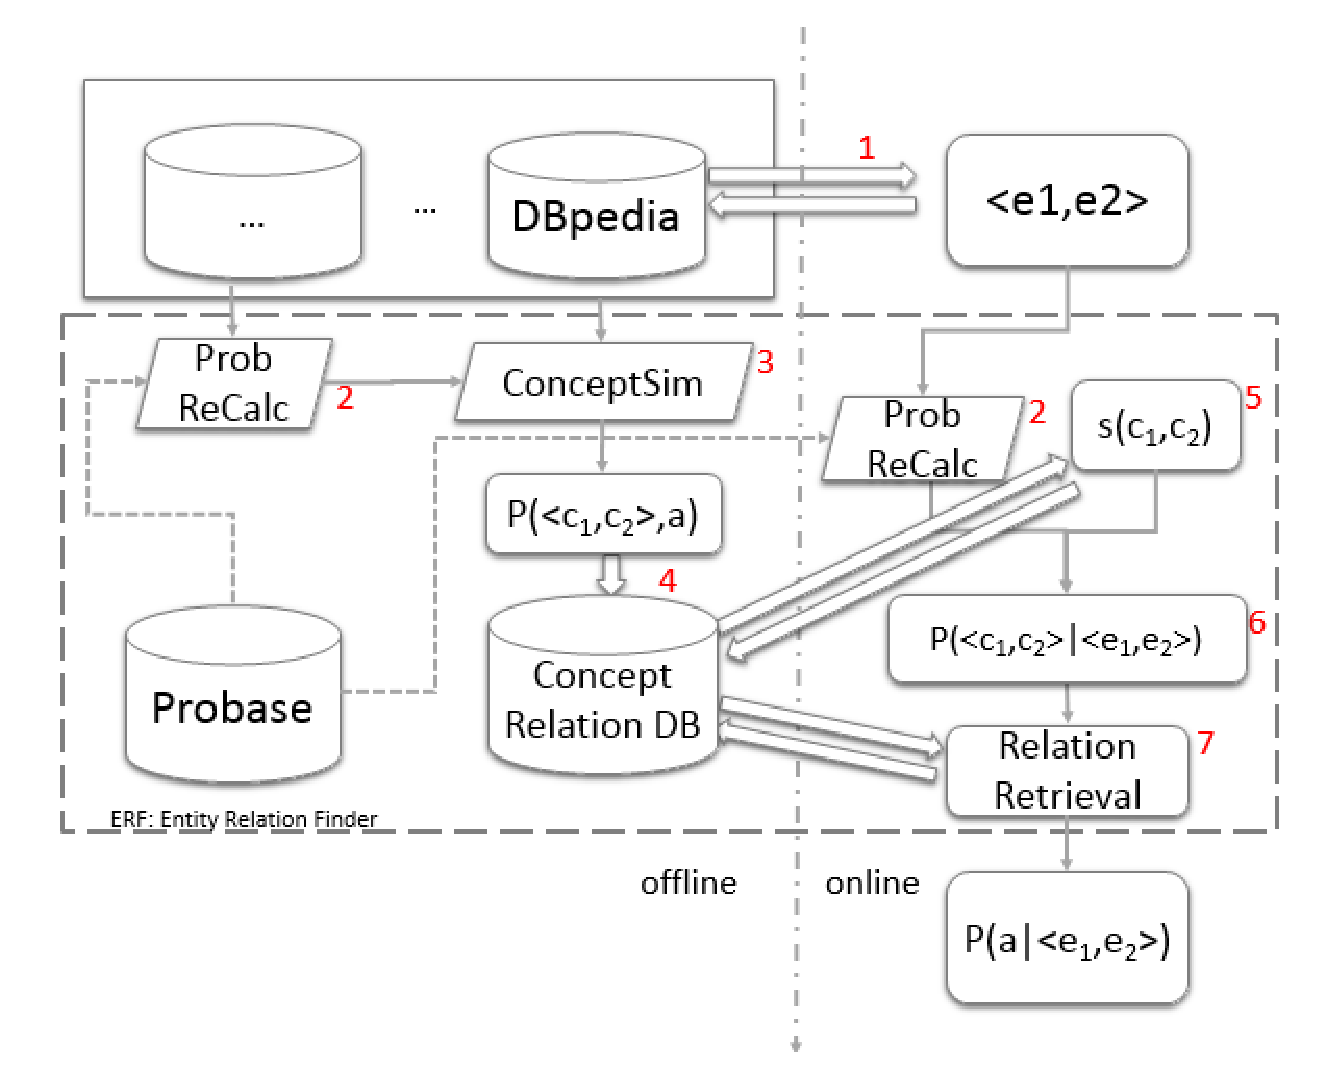
\epsfig{file=resources/framework.eps,width=0.8\columnwidth,height=0.5\columnwidth}
\vspace{-4mm}
\caption{System Framework of $ERF$}
\label{fig:framework}
\vspace{-6mm}
\end{figure}


%\nop{
%In the online part, we first directly lookup the attribute for the query entity pair from DBpedia.
%If DBpedia has no the exact the SPO triples connecting the entity pair, we In $step 2$, the concepts of the entities in knowledge bases are calculated(i.e. $P(c_i|e_i)$ in Eq.~\ref{eq:target_expand2_jr}).
%The detailed process in in
%$Step 3$ is the training process, $P( \langle c1,c2 \rangle ,a)$ is calculated for every attribute $a$ in Eq.~\ref{eq:pccga}.
%The result is then stored in Concept Relation DB in $step 4$.
%
%In  $step 1$, when a query entity pair comes, knowledge bases such as DBpedia are looked up and the exact relationship, if exists, is answered in the first place.
%If nothing is found in $step 1$, the process will go into the $ERF$ solution.
%
%We first conceptualize the 2 entities in $step 2$.
%The concept similarity score in Eq.~\ref{eq:target_expand2_jr}) is retrieved from the Concept Relation DB in $4$.
%%\ref{eq:pcca}
%So far we get everything for calculating Eq.~\ref{eq:target_expand2_jr}).
%Then in $step 7$ we query the concept relation database and get the relation between concept pairs, specifically, $P(a| \langle c_1,c_2 \rangle )$ in Eq.~\ref{eq:target_expand1}.
%Finally, we achieve the final object by combining all these together to infer $\argmax P(a| \langle e_1,e_2 \rangle )$ from Eq.~\ref{eq:target_expand_all}.
%We return the the attribute owning the maximal score as the explanation for the relationship between the entity pair.
%
%When no direct edges are found, we use the shortest path on the concept attribute graph to find the middle concepts, then the problem automatically reduced to relation explanation of several pairs of entities, discussing which is beyond the coverage of this paper.
%}


%\paragraph{Paper Orgnization}
%The rest of the paper is organized as follows, Section~\ref{sec:conceptualization} describe how to derive $P(c|e)$ leveraging the \xch{basicness} of concept, Section~\ref{sec:fafa} is devoted to the offline calculation of $JD(c_1,c_2)$ and $P((c_{1},c_{2})|a)$.
%\renewcommand\baselinestretch{-6}\selectfont
\renewcommand{\arraystretch}{-2}
%
%\begin{table}[htbp]
%  \centering
%     \small
%  \caption{Notation Table}
%    \footnotesize
%
%    \begin{tabular}{|ll|ll|}
%    \hline
%    notation                            &  meaning                            & notation                            &  meaning  \\
%    \hline
%    $n(\cdot)$                          &  count of                            & $e_i$                               &  entity  \\
%    $h(\cdot)$                          &  head of                             & $c_i$                               &  concept  \\
%    $a$                                 &  attribute                          & $c_l$                               &  long concept  \\
%    $\bar{C}$                           &  head concept set                  & $c_h$                               &  head concept  \\
%    $\langle e_1,e_2\rangle$            &  entity pair                        & $\langle c_1,c_2\rangle$            &  concept pair \\
%    $\alpha(\cdot,\cdot)$               &  joint factor                       & $T_k$                               & \parbox{0.26\columnwidth}{ set of E$A$E tuple with $a_k$ as $A$} \\
%    \parbox{0.15\columnwidth}{\scriptsize $P(a|\langle c_{1},c_{2}\rangle)$ }  &  \parbox{0.24\columnwidth}{ the typicality of an attribute for a concept pair. }& \parbox{0.23\columnwidth}{\scriptsize $P(\langle  c_{i},c_{j}\rangle|\langle e_{1},e_{2}\rangle)$} & \parbox{0.26\columnwidth}{ the typicality of the concept pair for an entity pair} \\
%    \hline
%
%    \end{tabular}%
%
%  \label{tab:notation}%
%  \vspace{-6mm}
%\end{table}%
%
%\renewcommand{\arraystretch}{1}

%First,we do conceptualization.
%
%Next,Judge whether the 2 entities are conceptually same
%
%Then, there are 2 cases of the CanBeExplained function:
%
%\begin{itemize}
%\item Explain 2 conceptually similar entity
%
%\begin{table}[htbp]
%  \centering
%  \caption{conceptually similar entity}
%    \begin{tabular}{rr}
%    \toprule
%    entity & concept \\
%    \midrule
%    Steve jobs & Person \\
%    Bill Gates & Person \\
%    \bottomrule
%    \end{tabular}%
%  \label{tab:addlabel}%
%\end{table}%
%
%
%\item Explain 2 conceptually different entity
%% Table generated by Excel2LaTeX from sheet 'Sheet1'
%\begin{table}[htbp]
%  \centering
%  \caption{Add caption}
%    \begin{tabular}{rr}
%    \toprule
%    entity & concept \\
%    \midrule
%    Mona Lisa & Painting \\
%    Renaissance & Period \\
%    \bottomrule
%    \end{tabular}%
%  \label{tab:addlabel}%
%\end{table}%
%
%Note that the concept here are not unique.
%
%\end{itemize}
%
%
%Last, We rank all the explanations in each step.
%
%
%


\vspace{-2mm}
\section{Collective Conceptualization (Offline Learning)}
In this section, we elaborate how we estimate $P(a)$ and $P( \langle c_{1},c_{2} \rangle |a)$ from knowledge bases, which is the major task in the offline learning component. As we have claimed, our major idea is collectively conceptualize multiple EAE instances instead conceptualizing each instance independently.
% We also introduce computation of $P(a)$ is another important part of the offline component.

\vspace{-2mm}
\paragraph{Collective Conceptualization ($P( \langle c_{1},c_{2} \rangle |a)$) }
We use SPO triples in DBPedia to compute the probability.
%We use these entity-attribute-entity instances to estimate the conditional probability of a concept pair given an attribute. 
The key of the computation is to assign a larger value for the true concepts pairs than false concept pairs.
For a certain attribute $a_k$, there are many entity pairs connected by the attribute in DBpedia, which allow us to aggregate the support from all entity pairs.
The aggregated score helps identify the true concept pair attribute to these properties:
\begin{enumerate}
\small
\item \emph{A false concept pairs are only supported by quite a few
entity pairs that have the attribute.}
\item \emph{A true concept pair in general is supported by most entity pairs of the attribute.}
\end{enumerate}

More formally, let $ \langle e_i, a_k, e_j \rangle $ be a SPO triple in DBPedia.
%The triple means that entity $e_i$ has a attribute $a_k$ with value or object as $e_j$.
%We only consider the SPO triples with O as entity, this attributes such as \at{height,year} are removed in the first place. 
Let $T_k=\{\langle e_i, a_k, e_j \rangle\}$ be all the triples in DBpedia with attribute as $a_k$.
$P( \langle c_1, c_2 \rangle |a_k)$ is estimated as follows:
\begin{equation}
\small
P(\langle c_1, c_2\rangle|a_k)= \frac{1}{|T_k|}\sum_{  (e_{i},a_k,e_{j})\in T_k } P(c_1|e_{i})P(c_2|e_{j})
\label{eq:pccga}
\end{equation}
It is not difficult to prove that $0\leq P( \langle c_1, c_2 \rangle |a_k)\leq 1$ and their sum over all concept pairs equals to 1.
Hence $P( \langle c_1, c_2 \rangle |a_k)$ is a probability estimation.


{\footnotesize
\begin{example}[Calculating $P( \langle {c_h}_{1},{c_h}_{2} \rangle  |a)$]
\label{exa:pggga}
Figure~\ref{fig:bipartite} shows many entity pairs of attribute \at{FoundedBy}. 
We can see that the false concept such as \at{fruit} is supported by only \at{Steve Jobs}.
However, the true concept pair \at{<company, entrepreneur>} is supported by all the three concept pairs. 
By summing up all $P(c_1|e_1)P(c_2|e_2) $ over all entity pairs, the true concept pair \at{<company, entrepreneur>} has a significant larger score than the false one \at{<fruit, entrepreneur>}.
\end{example}
}


%\vspace{-2mm}
\begin{figure}[!htb]
\vspace{-6mm}
\centering
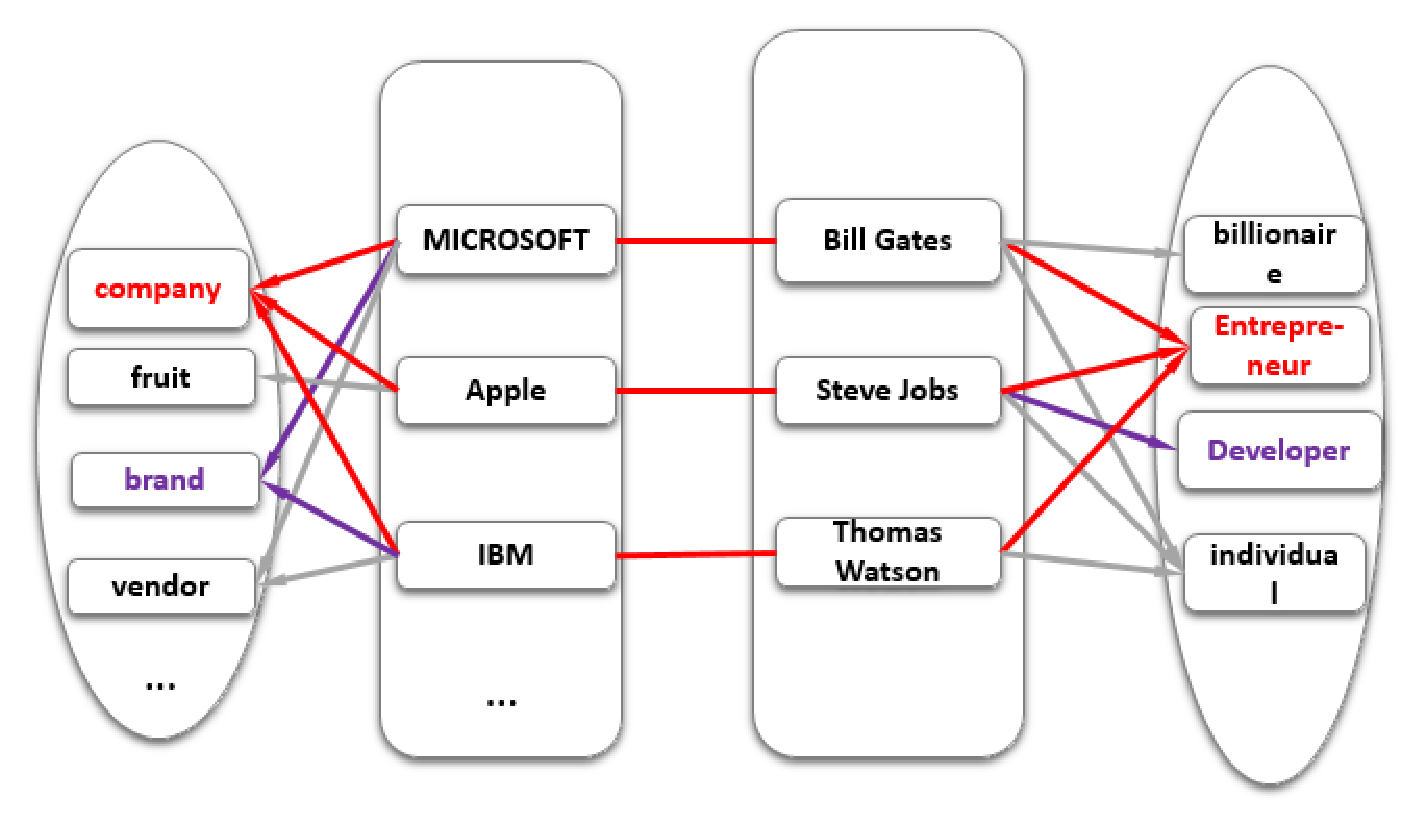
\epsfig{file=resources/ceaec.eps,width=\columnwidth, height=0.4\columnwidth}
\vspace{-8mm}
\caption{Calculating $P(  \langle {c}_{1},{c}_{2} \rangle  | \term{FoundedBy} )$ }
\label{fig:bipartite}
\vspace{-3mm}
\end{figure}

\vspace{-2mm}
\paragraph{Computation of $P(a)$}
For a given attribute $a$, $P(a)$ can be computed by
$
P(a)=\frac{n(a)}{\sum_{a_k\in A}{n(a_k)}},
$
where $n(a)$ is the count of triples in DBpedia with attribute $a$.
Note that only we only use SPO triples where both S and O are entities.


%\nop{
%\paragraph{Complexity analysis}
%
%We first analysis the complexity of calculating $P(\langle c_i, c_j \rangle|a_k)$, manifest in Table.~\ref{tab:complexity}. The original one need to calculate $P(\langle c_i, c_j \rangle|a_k)$ for all $c \in C_1,C_2 $,while most of the concepts are, according to the power law, close to zero, which indicates the rationality of pruning.
%
%
%\begin{table}[htbp]
%  \centering
%  \caption{Complexity Analysis}
%    \begin{tabular}{rr}
%    \toprule
%    method & complexity \\
%    \midrule
%    original &  $O(|T_n||C_1||C_2|)$ \\
%    topKpruned & $O(|T_n|K^2)$ \\
%    \bottomrule
%    \end{tabular}%
%  \label{tab:complexity}%
%\end{table}%
%}






%%% Local Variables:
%%% mode: latex
%%% TeX-master: "main.tex"
%%% End:

\vspace{-2mm}
% !TEX root = main.tex
\section{Conceptualization for Relationship Explanation}
\label{sec:conceptualization}
In this section, we give our solution to compute $P(c|e_i)$, the probability that $c$ is a concept of entity $e_i$.
We use Probase, a web-scale taxonomy, for the computation. We first briefly introduce Probase and give a direct solution. However, the direct conceptualization solution ignores the unique setting of relationship explanation. We will analyze the problems caused by our problem setting then give an improved version.problem here is that

\subsection{Problem Statement}
\yh{Probase exploit Hearst patterns to extract isA relations from 1.68 billion web pages . For example, it extracts evidence for the claim \at{IBM \isa company, Nokia \isa company} from sentence \at{...\ac{companies} such as \ac{IBM, Nokia}...}
is an instance of the concept president. The core version
of Probase contains 3,024,814 unique concepts, 6,768,623
unique instances, and 29,625,920 isA relations.}

Given an entity $e$, from Probase, we can acquire its concepts' set $C(e)$. For each $c_i \in C$, the frequency $n(c_i,e)$ can be accordingly derived, which means how many times the $e$ isA $c$ can be observed from the corpus. The frequency information allows us to estimate  $P(c|e)$ by
$$P(c|e)=\frac{n(c,e)}{\sum_{c_i\in C(e)}n(c_i, e)}$$


\paragraph{Refinement by Head Concepts}
We further argue that the relationship between entities are determined by the head concepts. For example, the \at{founder} relationship between \at{Apple Inc.} and \at{Steve Jobs} are determined by the head concepts they possessed (e.g.\ \term{company} and \term{entrepreneur}, regardless of the modifiers such as \term{technology} in the concept \term{technology company}.) Hence, the attribute should be generated by the head concept pair instead of the concept pairs with modifiers. This motivates us to refine the optimization objective by summing over on the head concept pairs. Let $\bar{C}_1$ and $\bar{C}_2$ be the head concepts in  $C_1$ and $C_2$, respectively. Our problem is refined as:
\begin{equation}
\label{eq:target}
\argmax_a \sum_{c_i\in \bar{C}_1 , c_j \in \bar{C}_2 }P(a|<c_{i},c_{j}>)\times P(<c_{i},c_{j}>|<e_{1},e_{2}>),
\end{equation}

By restricting the concept to the head concept, we can further reduce the computation cost.
The number of head concept pairs is obviously significantly smaller than that of the concept pair and that of entity pairs. Because most concepts are tail concepts with long modifiers. Head concept allows us to find the limited number of relationships without handling the huge number of long-tailed concepts and their entities.

\paragraph{Conceptualization into Head Concepts}

Given a head concept $c_h$, we need to estimate $p(c_h|e)$. However, we are likely underestimate $p(c_h|e)$ because in genereal there is no sufficient direct isA relationships from entity $e$ to the head concept $c_h$. We illustrate this in Example~\ref{exa:conc}. For our task, we only need relatively general concepts(a.k.a. head concepts).
\begin{example}[Underestimation of head concept]
\label{exa:conc}
Consider the entity \ac{Mona Lisa}. Its concepts in Probase include \ac{\{painting, famous painting, world's most famous painting\}}. The frequency between \ac{Mona Lisa} and each concept are\term{33,8,1}, respectively. The isA link from \at{Mona Lisa} and \ac{Painting} is missing since we always talk about \at{Mona Lisa} as a famous painting. Directly using the data in Probase, we have $$P(\ac{Painting}|\at{\text{Mona Lisa}})=0$$, which is obviously an underestimation.
\end{example}


For each entity $e$, we first retrieve all concepts of $e$ in Probase. Let the set of these concepts be $C(e)$. Then, we reduce $C(e)$ to $\bar{C}(e)$ so that each concept in $\bar{C}(e)$ contains all head concepts of each concept in $C(e)$. \yh{We identify the head concept by syntax-based patterns~\cite{ponzetto2007deriving} for NP .}. We denote each head concept as $c_h$ and the concept with modifiers as $c_{l}$ are the rest. Our problem is reduced to the recalculation of the probability $P({c_h}|e)$.
\yh{in experiments, we should compare the baseline that directly use concepts instead of head concepts.}



\begin{example}[Head concepts VS Original concepts]
\label{exa:HvsO}
Take \term{famous painting} as example. Its original concepts are \term{image, treasure}, which are reasonable but not plausible, since their occurrence are 2 and 1 respectively. However, the most plausible concept \term{painting} is not among the concepts.
\end{example}

\yh{Rewrite the objective function when we only consider the head concepts}

\paragraph{The main steps}
Given an entity $e$ from $Probase$, we can get its concepts from probase. First we do head modifier detection based on syntax[], since the concepts in Probase all follows English grammar, this approach already produces a good result. Next, we recalculate the probability of $P({c_h}|e)$ by aggregating the contribution from $c_l$. The essentiality of doing so is illustrated in Example~\ref{exa:recalc}. Finally, we provide a method to take the original isA relation from Probase into consideration.




\begin{example}[Essentiality of Aggregation]
\label{exa:recalc}
\term{steve jobs} The concept\term{well-known name} has four occurrences however \term{name} has only 2. There are other modifiers for the same head, so that the typicality of the head will be largely underestimated.
\end{example}



\subsection{Baseline}

The basic idea of the improved estimation is aggregating the information of all subconcepts of the head concepts.  We should contribute all the counts of $C_{l}$ to $C_{simple}$.


After head modifier detection, we have a set of ${c_h} \in C_{simple}$, among all the $c_{l_j}\in C_{l}$, there are 2 cases in the probase determined by whether the $c_{l_j}$ has an isA edge towards ${c_h}$ or not.
The intuition of doing so is illustrated in the Example~\ref{exa:clc}:

\begin{example}[contributing long concepts]
\label{exa:clc}
Assume that  \term{Mona Lisa is a painting} and \term{Mona Lisa is a famous painting} are observed respectively \term{33 times and 8 times} from different documents, we will get the knowledge that \term{Mona Lisa is a painting} occurs \term{41 times} instead of \term{33 times}.
\end{example}

Hence, the most straight forward approach is to contribute the corresponding long concepts to the simple ones as follows:

$$\hat{n}(c_h, e)={n}(c_h, e)+\sum_{ h(c_l)=c_h} n(c_l,e)$$
$$\hat{P}(c_h|e)=\frac{\hat{n}(c_h, e)}{\sum_{c_{h'}}{\hat{n}(c_{h'}}, e)}$$
where $f_{HM}()$ is a function that takes a long concept and produce a head concept.
....... Head concept space, typicality....
\yh{rewrite example}


\subsection{Combined Model with Original IsA}
When obtaining $\hat{P}(c_h|e)$, we are in fact judging the typicality of a concept.
In this section, we take the original Probase IsA relation into consideration. In Example.~\ref{exa:isagood}, we can observe some reasonable results produced by the Probase isA relationship.

\begin{example}[Resonable isA Relation]
\label{exa:isagood}
  There exists several original IsA concepts of the long concepts that are also reasonable. For example \term{ topaz}(a kind of yellow gemstone) has the concept \term{precious stones}, and \term{precious stones} has an edge towards \term{material} which is reasonable.
\end{example}

Based on the how to treate $c_l$, we have the following 2 cases:

\begin{description}
  \item[$c_l$ appear as an concept] In this case the counts that its entities produced should be take into consideration into $c_h$, deriving the following Case A.
  \item[$c_l$ appear as an instance] In this case $c_l$ is observed from the corpus as an instance at the left side of an isA sentence, it should be treated the same as other entities $e$, deriving the following Case B.
\end{description}


Therefore, to calculate  $P({c_h}|e)$, there are three cases.:

\begin{description}

\item[Case A.1 $e$ \isa ${c_h}$ ]
 The entity has has an isA edge towards one or more simple concept, which gives the original $P_{org}({c_h}|e)=$


\item[Case A.2 $e$ \isa $c_{l}$ \noisa ${c_h}$]  The solid edge here refers to the isA relationship in $Probase$ and the dashed one refers to the edge generated by head modifier detection. Example~\ref{exa:wahro} pointed out that there won't be necessarily an isA edge from \term{famous painting}($c_{l}$ ) to \term{painting}(${c_h}$), however $c_{l}$ is obviously a hyponym of ${c_h}$. In this case,
    % since it's detected by the head modifier method, we assume
    % $$P_{head}({c_h}|c_{l_j})=1 $$
    we have to re-calculate the $P({c_h}|{c_l})$.
    In the original probase approach, we use Eq.~\ref{phgl_org} to calculate the probability.
    \begin{equation}\label{phgl_org} P({c_h}|{c_l}) = \frac{n( {c_h},{c_l} )}{ \sum{n( {c_h}^*,{c_l} )}  } \end{equation}
    However, $n( {c_h},{c_l} )$ is lower than expected due to the reason demonstrated in Example.~\ref{exa:wahro}.
    Therefore, we alternatively utilize the $\sum{ e^*,n({c_l}) } $ as the occurrence of $c_l$, following the assumption that \em{ whether $c_l$ is typical towards its $c_h$ is independent from }
    $$P_{head}(c_h|e)=\frac{\sum_{c_h= f_{HM}(c_l*)} n(c_l*,e)}{ n(e)} $$

\item[Case B $e$ \isa $c_{l}$  \isa ${c_h}$]  In this case, we need to calculate the following equation
$$P({c_h}|e) = \sum_{c_{l}^*\in C_{l}}   P({c_h}|c_{l}^*,e)   \times    P(c_{l}^*|e) $$
, where $P(c_{l}^*|e)$ can be obtained from $Probase$ and
\begin{equation}P({c_h}|c_{l},e) = \frac{n({c_h},c_{l}, e)}{n({c_h}, e)}\label{eq:pcge}\end{equation}
We assume that the occurrence of $e$ does not affect $P({c_h}|c_{l})$ equivalently speaking, $P({c_h}|c_{l})$ is independent from $e$, thus Eq.~\ref{eq:pcge} can be simplified
$$P({c_h}|c_{l},e) =P_{probase}({c_h}|c_{l}) = \frac{n({c_h},c_{l})}{n({c_h})}$$
which can be obtained from $Probase$.

\end{description}

\begin{example}[Why aren't head relationship observed]\label{exa:wahro}
There are less chance of occurring \term{Famous painting is a painting} in the corpus, since human takes it for granted and will seldom express it in such a way, so that there won't be necessarily an isA edge from \term{famous painting} to \term{painting} in the KB, while we insist it is necessary.
\end{example}

%%%%%%%%%%%%%%%%%%%%%%%%%%%%%%%%%%
%\nop{
%In both case B.1 and B.2, the weight of the edge $c_{l}$ \isa ${c_h}$ is underestimated. We argue that when calculating the typicality $P({c_h}|e)$, the counts of the long concept contributing to its head concept should be re-estimated as follows.
%
%Notice that the boundary between case B.1 and case B.2 are not strict, there are such edges that have low observation in Example~\ref{exa:HvsO}. So that if we consider them as a whole, we can derive:
%\begin{equation} P({c_h}|c_{l})=\lambda P_{head}({c_h}|c_{l})+(1-\lambda)P_{probase}({c_h}|c_{l}) \label{eq:pcgclong}\end{equation}
%where $\lambda$ is a parameter \xch{principle: related to plausibility, number of occurrence, varies for different $c_{l}$ should it be derived from learning ?} since we assume $P_{head}({c_h}|c_{l})$ to be 1, Eq.~\ref{eq:pcgclong} is simplified to:
%$$P({c_h}|c_{l})=\lambda  +(1-\lambda)P_{probase}({c_h}|c_{l}) $$
%}
%%%%%%%%%%%%%%%%%%%%%%%%%%%%%%%%%%%%

Considering Case A.1 and Case A.2 we get the baseline. When calculating typicality, we should consider the both cases of $c_l$, thus combining Case A and B through a linear combination.

Finally  $P({c_h}|e)$ is calculated using the following equation:

\begin{equation}
\begin{split}
P({c_h}|e) = \alpha \hat{P}({c_h}|e)+ (1-\alpha) \sum_{ c_{l}^*\in C_{l} } [P({c_h}|c_{l}^*) ] \times  P(c_{l}^*|e)
\end{split}
\label{eq:pgge}\end{equation}






\begin{figure*}[!hptb]
\label{fig:pgge}
\centering
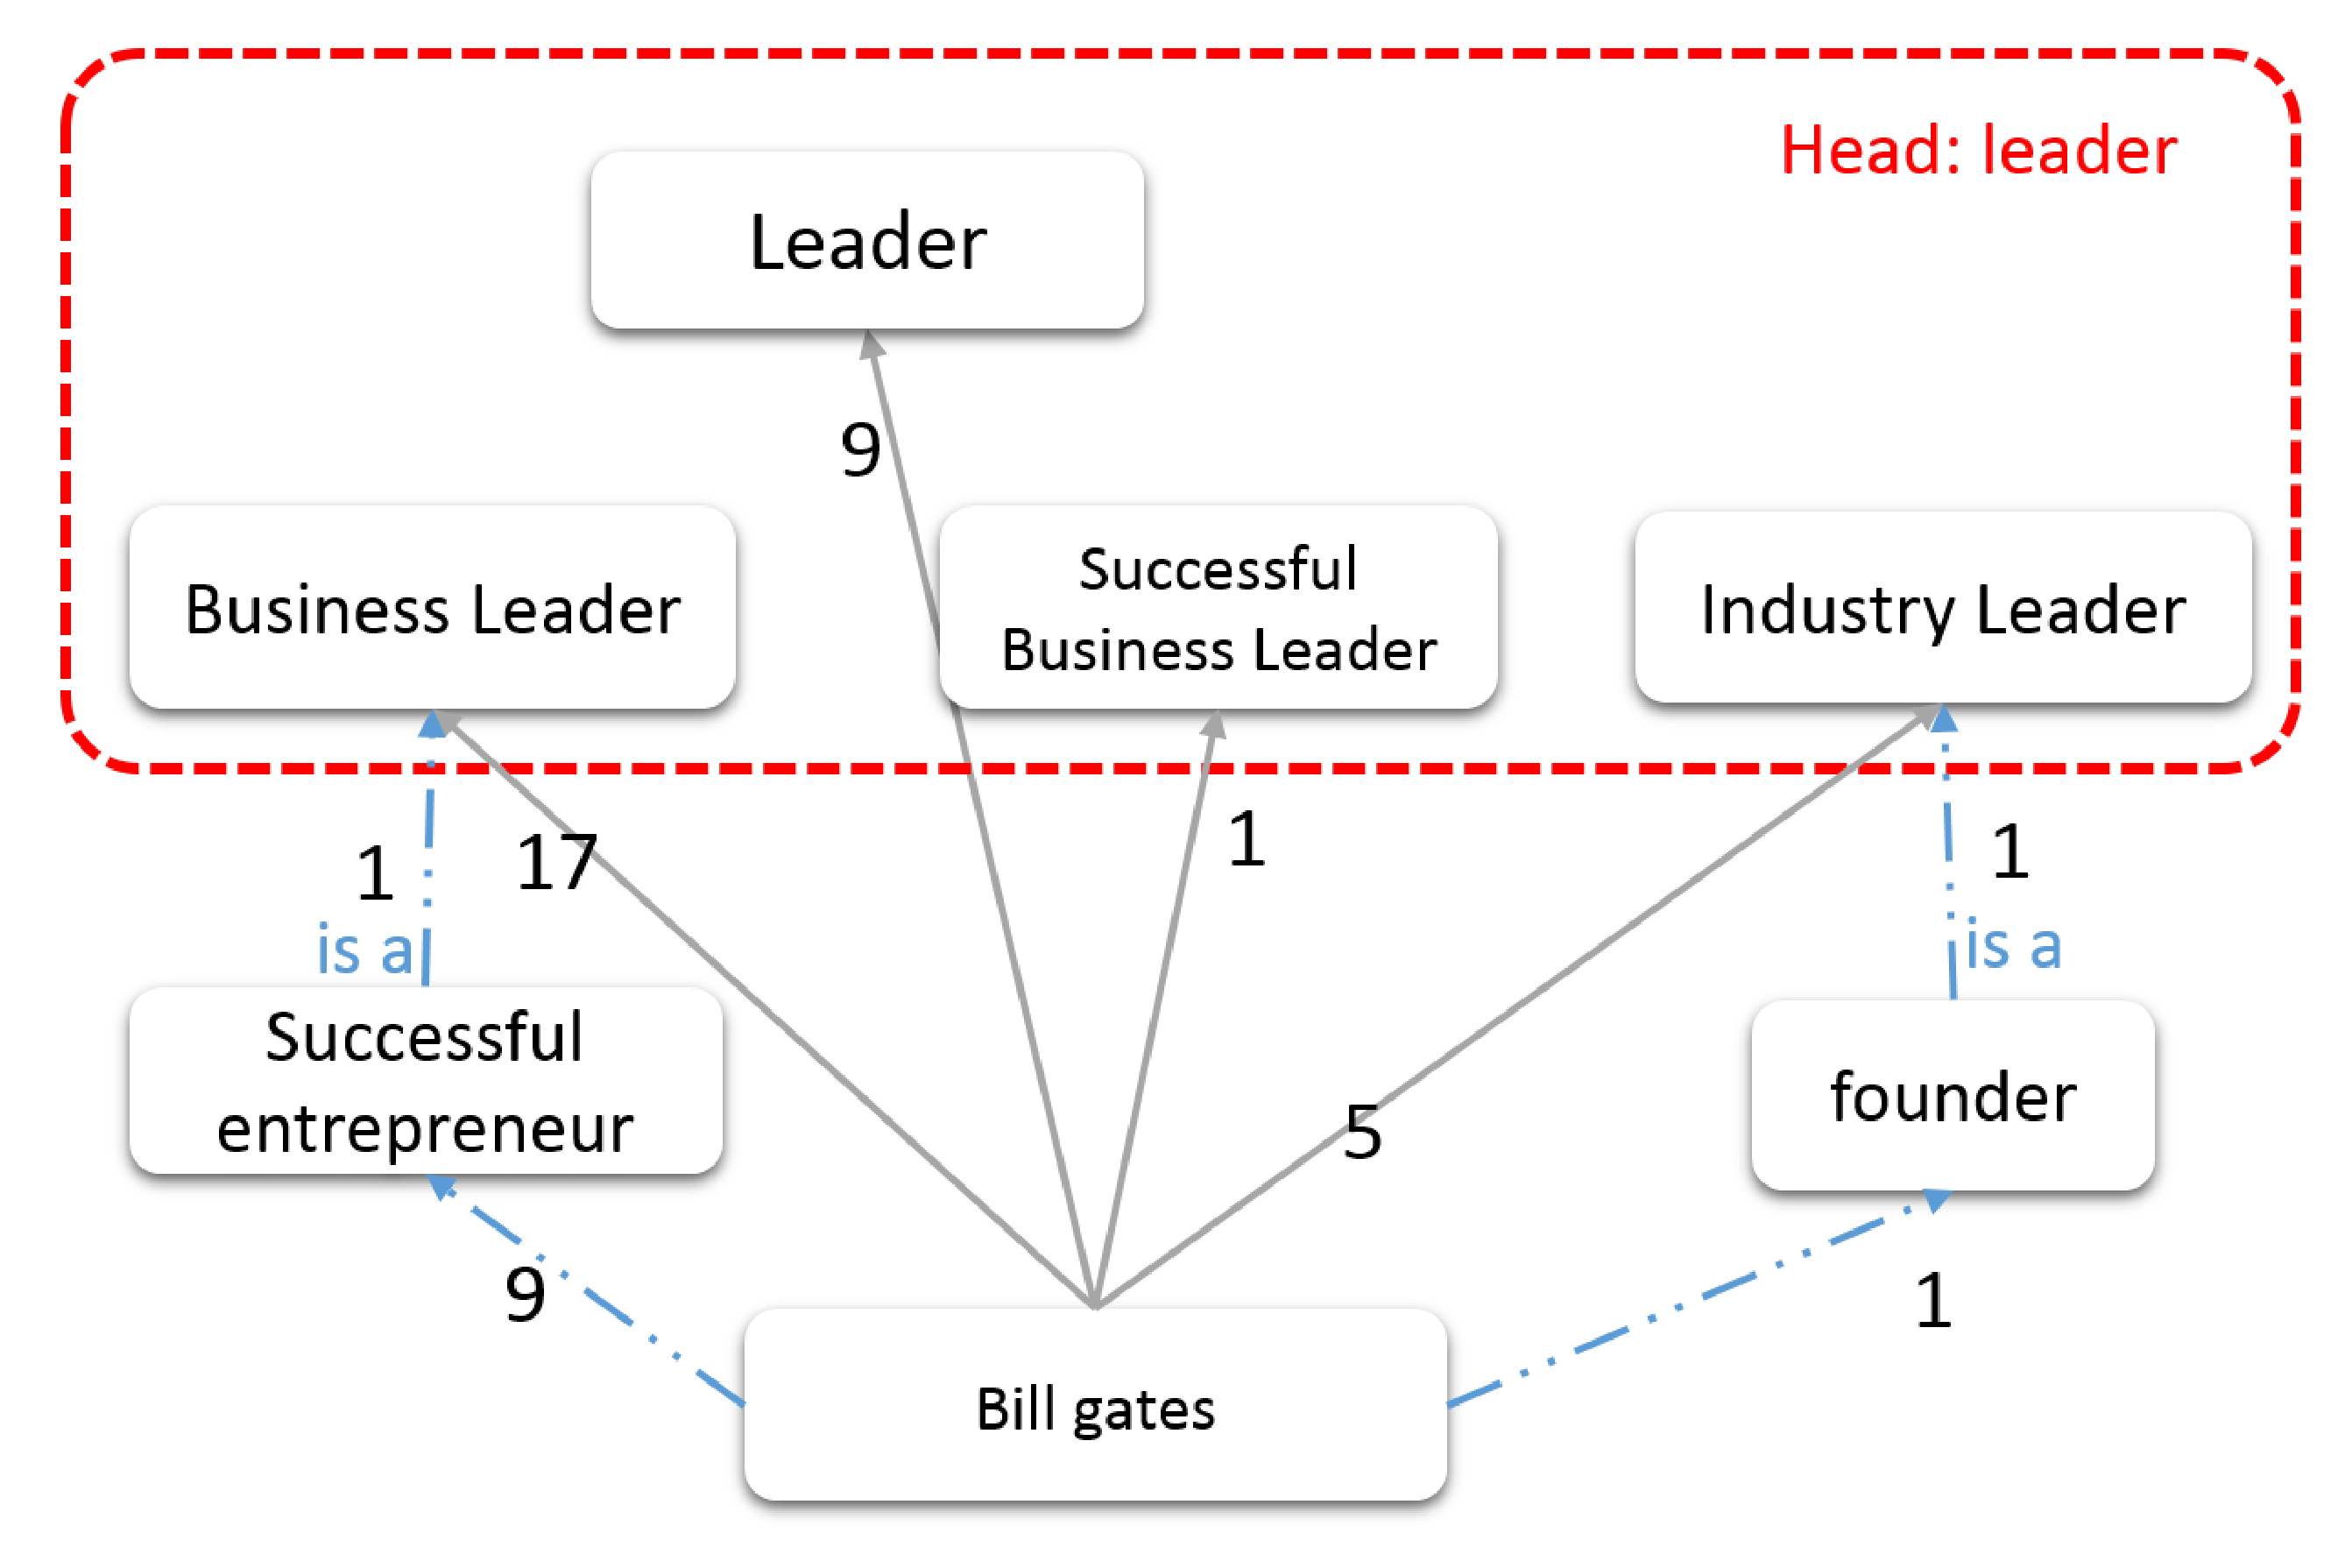
\epsfig{file=resources/bill_gates_isa.eps,width=5.5in}
\caption{calculating $P({c_h}|\term{Bill Gates})$ }
\end{figure*}


\nop{
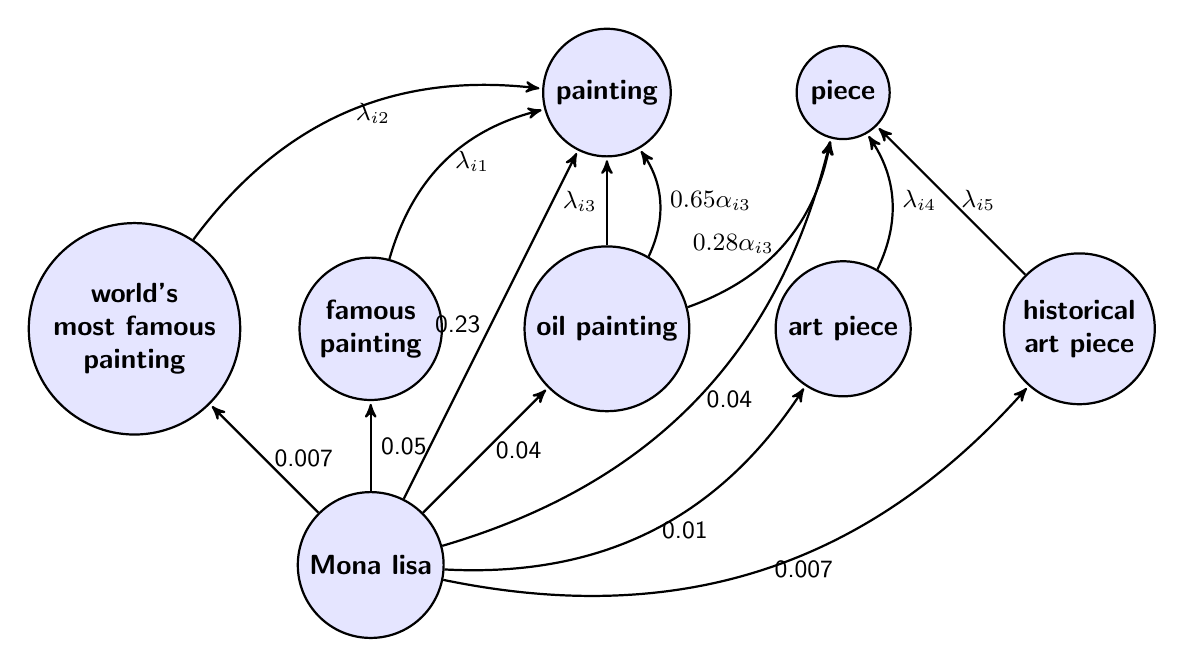
\begin{tikzpicture}[->,>=stealth',shorten >=1pt,auto,node distance= 3 cm,
  thick,main node/.style={circle,fill=blue!10,draw,font=\sffamily\bfseries,align = center}]

  \node[main node] (4) {piece};
  \node[main node] (2) [left of=4] {painting};

  \node[main node] (5) [below of=2] {oil painting};
  \node[main node] (6) [left of=5] {famous\\painting};
  \node[main node] (7) [left of=6] {world's\\most famous\\painting};

  \node[main node] (10) [right of=5] {art piece};
  \node[main node] (11) [right of=10] {historical\\art piece};

  \node[main node] (12) [below of=6] {Mona lisa};


  \path[every node/.style={font=\sffamily\small}]

    (5) edge  node [left] {$\lambda_{i3}$} (2)
        edge [bend right] node [right] {\small{$ 0.65\alpha_{i3} $}} (2)
        edge  [bend right] node[left]  {\small{$ 0.28\alpha_{i3} $}} (4)
    (6) edge [bend left] node [right] {$\lambda_{i1}$} (2)
    (7) edge [bend left] node [right] {$\lambda_{i2}$} (2)

    (10) edge [bend right] node[right] {$\lambda_{i4}$} (4)
    (11) edge node[right] {$\lambda_{i5}$} (4)
    (12) edge [bend right]node[right] {0.01} (10)
         edge [bend right]node[right] {0.007} (11)
         edge node[right] {0.04} (5)
         edge node[right] {0.05} (6)
         edge node[right] {0.007} (7)
         edge node[left] {0.23} (2)
         edge [bend right]node[right] {0.04} (4);

\end{tikzpicture}
}


%
%The process of calculation is illustrated in the example~\ref{exa:calc}
%
%\begin{example}[Calculating $P({c_h}|e)$]
%\label{exa:calc}
%As illustrated in Fig.~\ref{fig:pgge}, the process of calculating the typicality a concept is as follows, where \term{painting} is ${c_h}$ and \term{Mona Lisa} is $e$. Then $P(\term{painting}|\term{Mona Lisa})$ consists of 2 parts, the direct edge $P_{original}({c_h}|e)= 0.23$, and the second part
%$$\sum_{ c_{l}^*\in C_{l} } [ \lambda_{i}^*+(\alpha_{i}^*) P({c_h}|c_{l}^*) ] \times  P(c_{l}^*|e) $$
%$(\alpha_i^*+{c_h}^*=1)$
%Thus we get
%$$ P = 0.007\times \lambda_{i2}+0.05\times \lambda_{i1}+0.04\times(\lambda_{i3}+0.65\alpha_{i3}) $$
%For \term{piece}, it is the similar process. The relation here is only part of the whole graph.
%\end{example}




We consider only 2 layers of isA relationship for 2 reasons. The first one is that more layers will lead to noisy concepts such as \term{issue, factor, element}, which are concepts for almost eveything, Secondly, discussing the transitive relation between concepts is beyond the scope of this paper.

%% !TEX root = main.tex
\section{Find Alias For Concepts}
\label{sec:fafa}

%For a pair \term{(Sherlock holmes, United Kindom)}, \term{country} is a merely-ok attribute, on the contrary, \term{residence, deathPlace} are better since they are more specific and more seemingly plausible to be an attribute.
%We argue that for each pair of entity, there is a selectional preference for attribute.


%where $f()$ denotes the importance of a concept itself, $g( , )$ denotes the joint ratio of the concepts.
% ENERGY_FUNCTION( f(c1) * f(c2) * g(c1,c2) )


This section is devoted to calculating $s(c_1,c_2)$ of $P(<c_{1},c_{2}>|<e_{1},e_{2}>)$ in Eq.~\ref{eq:target_expand2_jr} and $P(<c_{1},c_{2}>|a)$ of $P(a|<c_{1},c_{2}>)$ in Eq.~\ref{eq:target_expand1}.

According to $P(<c_1,c_2>|<e_1,e_2>)$, we can only at concept level indicate the implicit relationship.
$P(a|<c_{1},c_{2}>)$ retrieves the most probable alias of relation given the concept pair.
Thus our objective function solve 2 problems,
1) give out the most probable relation alias for a concept pair.
2) when multiple relations exist in one concept pair, decide which one is most typical.

One simple version of the objective function derived from Eq.~\ref{eq:target_expand_all} is equal to Eq.~\ref{eq:simple_obj} when Eq.~\ref{eq:rel_jdp} holds, where we consider $s(c_1,c_2)$ to be how likely the two concepts are going to co-occur.

\begin{equation}
\label{eq:simple_obj}
 \argmax_a \sum_{c_i\in C_1, c_j\in C_2} p((c_{i},c_{j})|a) P(a) P(c_i|e_1) P(c_j|e_2)
\end{equation}

\begin{equation}\label{eq:rel_jdp}
  s(c_1,c_2) = \sum{ P((c_{1},c_{2})|a^*) \times P(a^*)}
\end{equation}

%\xch{(c1,c2) is only one aspect, any other factor can affect the relation?}
%\xch{ in s(c1,c2), we only considered the attribute part, other signals such as entity co-occurrence of <e1,e2> can be considered }


Eq.~\ref{eq:simple_obj} means finding the most probable attribute of $(e_1,e_2)$ by looking at their best concept pair, and find the most probable attribute given the concept pair.


\subsection{ Concept Joint Ratio.}

$s(c_1,c_2)$ stands for the how likely for $c_1$ and $c_2$ to become a concept pair to depict entity relation.
This step, as mentioned before, is mainly for concept level disambiguation purpose.

Let $T_n=\{(e_i, a_k, e_j)\}$ be all the triples in the knowledge base.
Eq.~\ref{eq:pcca} denotes the relation of joint probability of the pair $<c_1,c_2>$ and $a$.
\begin{equation}
P(<c_1, c_2>,a) = \frac{1}{|T_n|}\sum_{  (e_{i},a_k,e_{j})\in T_n } P(c_1|e_{i})P(c_2|e_{j})
\label{eq:pcca}
\end{equation}

To get $P(<c_1,c_2>)$ i.e( s(c1,c2) ), we sum up all the attributes in Eq.~\ref{eq:pcca}:
$$ s(c_1,c_2) = \sum_{a\in A} P(<c_1,c_2>,a)  $$



%\begin{definition}[Definition of $s(c_1,c_2)$]
%  $$ JD(c_1,c_2) = \frac{1}{Z_\theta}\times e^{- \frac{1}{f(c_1)\times f(c_2)\times g(c_1,c_2))}},$$
%  where $$f(c_i)=\sum{ P(c_i|e^*) },(i=1,2)$$
%  denotes the typicality of a concept itself, $$g({c_h}_1 ,{c_h}_2 )=\sum P({c_h}_{1}|e_{1i}^*) \times P({c_h}_{2}|e_{2j}^*)$$
%  denotes the joint ratio of the concepts.
%\end{definition}
%

\subsection{Calculating $P(<c_{h1},c_{h2}>|a)$ }


Given a set of concept pairs $ < {c_h}_1 , {c_h}_2 > $, where ${c_h}_1\in \bar{C}_1$ and ${c_h}_2\in \bar{C}_2$, we want to find a set of attributes A, where for each $a \in A$:
we can form $ <{c_h}_1,a,{c_h}_2 >$ tuple which best describe the relation between ${c_h}_1$ and ${c_h}_2$.

For a certain attribute $a_k$, there are many entity pairs of the attribute.
Let $T_k=\{(e_i, a_k, e_j)\}$ be all the triples in the knowledge base with attribute as $a_k$.
\begin{equation}
P(<c_1, c_2>|a_k) = \frac{1}{|T_k|}\sum_{  (e_{i},a_k,e_{j})\in T_k } P(c_1|e_{i})P(c_2|e_{j})
\label{eq:pccga}
\end{equation}

\begin{example}[Calculating $P(<{c_h}_{1},{c_h}_{2}> |a)$]
\label{exa:pggga}
As illustrated in Fig.~\ref{fig:bipartite}, the process of calculating $P(({c_h}_{1},{c_h}_{2}) |a)$ is as follows.
Given \term{company} and \term{entrepreneur}, we sum up all $P(c_1|e_1)\times P(c_2|e_2) $ such as $P(Company|Microsoft) \times P(Entrepreneur|Bill Gates)$,
\end{example}


\begin{figure}[!htb]
\centering 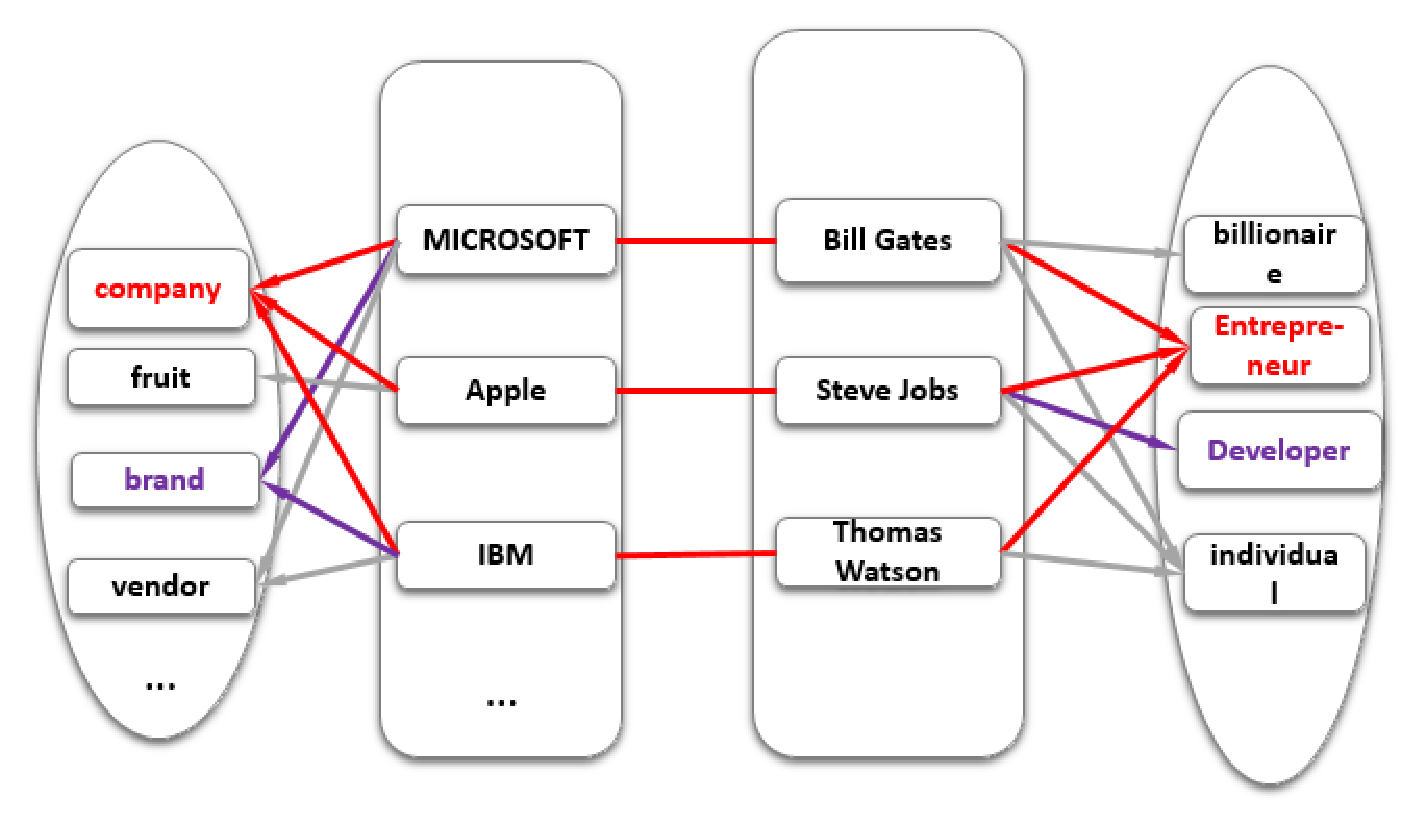
\epsfig{file=resources/ceaec.eps,width=\columnwidth}
\caption{Calculating $P( <{c}_{1},{c}_{2}> | \term{FoundedBy} )$ } \label{fig:bipartite}
\end{figure}





Let $C_1$ be all the concepts of $E_L(T_k)$.
Let $E_L(T_k)$ be all the left entities of attribute $a_k$ in the knowledge base.
We can prove that $\sum_{<c_i,c_j>\in C_1\times C_2} P(<c_i, c_j>|a_k)=1$.

\paragraph{Complexity analysis}

We first analysis the complexity of calculating $P((c_i, c_j)|a_k)$, manifest in Table.~\ref{tab:complexity}. The original one need to calculate $P((c_i, c_j)|a_k)$ for all $c \in C_1,C_2 $,while most of the concepts are, according to the power law, close to zero, which indicates the rationality of pruning.


\begin{table}[htbp]
  \centering
  \caption{Complexity Analysis}
    \begin{tabular}{rr}
    \toprule
    method & complexity \\
    \midrule
    original &  $O(|T_n||C_1||C_2|)$ \\
    topKpruned & $O(|T_n|K^2)$ \\
    \bottomrule
    \end{tabular}%
  \label{tab:complexity}%
\end{table}%



%To construct the Entity Attribute Graph, we only need topK concepts to form $({c_h}_1,{c_h}_2)$ pair, K trough \xch{case study} is around 5, so we here set K=10.
%
%tuple, later denoted as  $(e_1, a, e_2)$ , where $e_1$ and $e_2$ are also referred to as \term{domain} and \term{range} of the attribute. We can conceptualize $e_1$ and $e_2$ using the method in section~\ref{sec:conceptualization}, and get a set of concept $C_1,C_2$, accompanied with a set of probabilities $P({c_h}_{1}|e_{1i})$, $P({c_h}_{2}|e_2)$,where ${{c_h}_{1} \in C_1},{{c_h}_{2} \in C_2}$.
%
%
%Thus for any attribute $a$, given a pair of entity $(e_{1i},e_{2j})$, we can define:
%
%
%\begin{equation} \begin{split} P_{(e_{1i},e_{2j})}(({c_h}_{1},{c_h}_{2}) |a)&=P_{before}({c_h}_1|a) \times P_{after}({c_h}_2|a) \\&=  P({c_h}_{1}|e_{1i}) P(e_{1i}|a) \times P({c_h}_{2}|e_{2j})P(e_{2j}|a) \end{split} \label{eq:giga}\end{equation}
%
%
%where we use $P_{(e_{1i},e_{2j})}(({c_h}_{1},{c_h}_{2}) |a)$ to denote observing a single pair $(e_{1i},e_{2j})$, how likely is a combination of $({c_h}_{1},a,{c_h}_{2})$ to occur.
%
%
%
%
%Consequently,
%\begin{equation} P(({c_h}_{1},{c_h}_{2}) |a)=\sum_{  e_{1i} \in E_1 ,e_{2j} \in E_2} P_{(e_{1i},e_{2j})}(({c_h}_{1},{c_h}_{2}) |a) \label{eq:pg1g2ga}\end{equation}
%
%where $E_1,E_2$ denoting the whole set of domain entity and range entity,The  $P(e_{1i}|a)$ and $P(e_{2j}|a)$ here has only 2 values $1$ and  $0$, depending on whether  $e_1$ occurs before $a$ or $e_2$ occurs after $a$. Apparently, only $(e_{1i}, a, e_{2j})$ occurs will give the equation a non-zero value, therefore, Eq.~\ref{eq:pg1g2ga} is finally equal to Eq.~\ref{eq:gga_fin}.
%
%\begin{equation} \begin{split} P(({c_h}_{1},{c_h}_{2}) |a) &= \sum_{  (e_{1i},a,e_{2j})\in KB } P_{(e_{1i},e_{2j})}(({c_h}_{1},{c_h}_{2}) |a) \\&=  \sum_{  (e_{1i},a,e_{2j})\in KB }P({c_h}_{1}|e_{1i}) \times P({c_h}_{2}|e_{2j})\end{split} \label{eq:gga_fin}\end{equation}
%
%\xch{
%The process of calculating \term{} is demonstrated in Example.~\ref{exa:pggga}
%}
%






%
%\xch{ ==============problem here!!! the numerator and the denominator multiplies and get 1, is the relationship here correct??==========}
%
%We first specify the relationship between $P((c_{1},c_{2})|a^*) $ and $JD(c_1,c_2)$. Actually, they have the following relationship:
%\xch{===========================}


%To Construct the Entity Attribute Graph, we calculate $P(({c_h}_{1},{c_h}_{2}) |a)$ for each attribute.
%nOTE that we only consider the attributes whose range is an entity, and ignore those numerical values or date-and-time values such as $( Mona Lisa, Year, 1503)$.
%For each $({c_h}_{1},a,{c_h}_{2})$ tuple, we can calculate $P(({c_h}_{1},{c_h}_{2}) |a)$ for each



%\subsubsection{Voting}


%\subsection{For multiple hops}
%
%\subsubsection{Entity Attribute Graph Construction}
%
%
%\begin{figure}[!htb]
%\centering 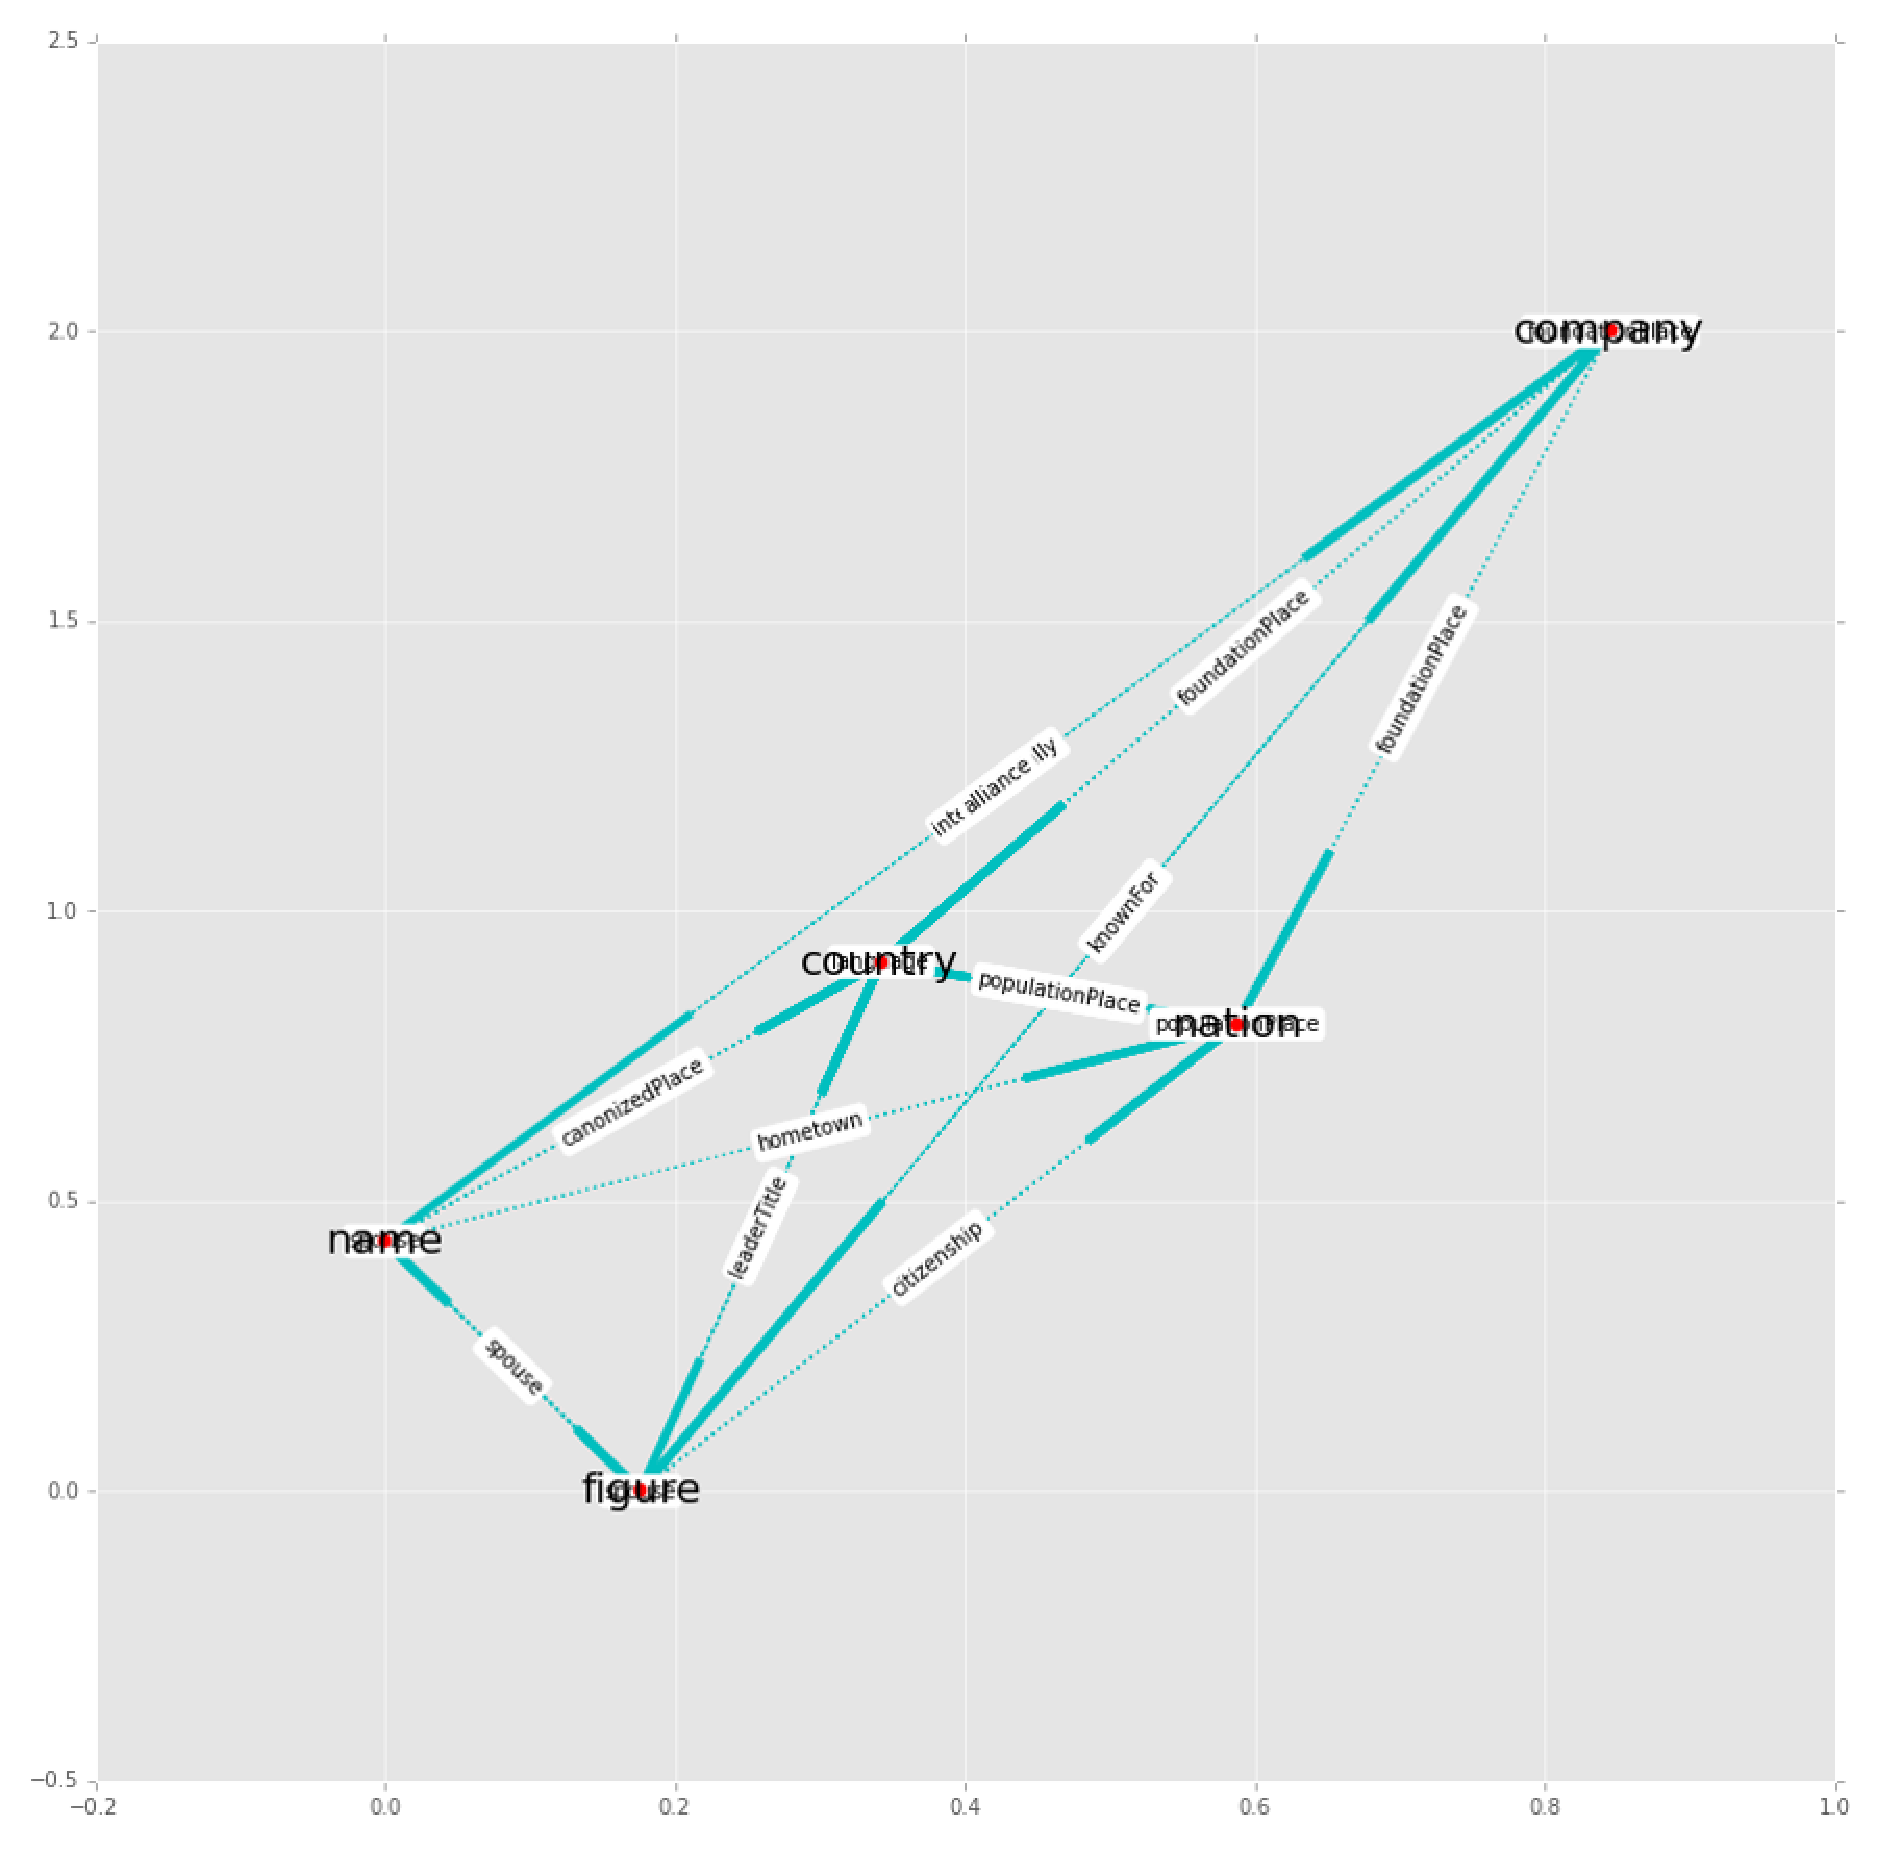
\epsfig{file=resources/eag.eps,width=2.5in}
%\caption{Subgraph of Entity Attribute Graph } \label{fig:eag}
%\end{figure}
%
%So far, we have tackled with the relations and generated the edges in the relationship graph.
%This problem is similar to {\bf hierarchy ranking problems in a directed graph}~\cite{gupte2011finding}. Originally, it was a minimum feedback arc set problem on a weighted network which is a classic NP-hard problem~\cite{dinur2005hardness}. A few approaches~\cite{tatti2014faster} have been proposed on unweighted directed graphs, for weighted graphs, the extended agony[hierarchies in directed network(unpublished kdd15)] algorithm can be ultilized to generate hierarchy results \xch{in this approach the K (number of hierarchies) is fixed, maybe we can make it adaptive to data here? }
%
%
%
%In this section, we first formulate the problem of finding semantic link into a maximum flow problem on the concept network with multiple-sources and multiple-sinks, and then, we cut out the subgraph and perform {\bf improved agony} to derive the concept of the middle entities. Last we use co-occurrence to verify the validness of the relation.
%
%%We argue that co-occurrences between entities can only be applied to entity relation explanation when they are conceptually correct[]. Following this intuition, we further formalize our problem into
%
%
%\subsubsection{Improved agony}
%
%



%\subsection{Find the best alias}
%
%We then Use an $\argmax$ model \xch{use KL divergence? to minimize $D_{KL}{}$} to solve the problem.
%
%Given $(e_1,e_2)$, our goal is to find the best attribute for it. We denote it as:
%$$\argmax P((e_1,e_2)|a) $$
%where
%$$P((e_1,e_2)|a)= $$


\vspace{-2mm}
% !TEX root = main.tex

\section{Experiments}
\label{sec:exp}

In this section, we present our experimental study.
We use DBpedia2014~\cite{dbpedia} and Probase~\cite{wu2012probase} as our knowledge repository.
We use entity pair as well as their attributes in DBpedia to learn the conceptual patterns.
We use Probase for conceptualization. We carry out all the experiments on a PC with Intel i7 cpu @2.5Ghz and 16G memory. All the programs are implemented in Python.

\paragraph*{Evaluation Metrics}
Given a pair of entities, our system produces the most plausible top-K attributes between them.
We need to evaluate how accurate the result is. 
Hence, we use $nDCG@K$ and $Precision@K$ as our evaluation metric.
We report the $MAP@K$ (Mean Average Precision at K) as well.
We further use $ ERR@K$~\cite{chapelle2009expected} to evaluate the {\it Expected Reciprocal Rank}, which is based on the user behavioral model emulating that a user would stop browsing if the first several ranked results are undesirable. In our collective conceptulization procedure, evaluating the correctness of first $K$ concept pairs is similar to user browsing case. In our case, a user may stop looking at more concepts if top-$K$ concepts already provide sufficient conceptual information for the entity pair.
% 我突然想到了我这里做过个优化, 每次算concept pairs 的时候按照P(C|E)排个序,如果排在后面的c,乘上最大的P(<c1,c2>|a)P(a)也不能超过前面的,就停止搜索了。2015年9月15日19:23:27


\subsection{Exp1: Effectiveness of $ERF$}
In this experiment, we evaluate the effectiveness of our ERF system.
We first show that ERF systems can explain relationship for most entity pairs.
We compare to a baseline that directly retrieves the attribute from DBpedia according to the entity pair.
We randomly select 50 Wikipedia article (entity $e_1$) and the hyper-linked entities in its abstract (entity $e_2$)
to construct query entity pairs.
The result is reported in Table~\ref{tab:precision_compare}.
Overall, ERF can generate correct attributes for 83\% entity pairs.
Our system explains 15.77\% more entity pairs than the baseline (64\%).

\nop{
Since we assume 0 if the entity has no relation can be retrieved from database and otherwise 1, the average $Precision@1$ results here can also be viewed as \ac{recall} of the knowledge base.
DBpedia provides only one relation for a covered entity pair, therefore we use $Precision@1$ to compare the results.
Our ERF method improves the average $Precision@1$ by 15.77\%.
}

\nop{
\begin{table}[htbp]
  \centering
  \caption{Precision@1 Compared With Baseline}
    \begin{tabular}{rrr}
    \toprule
         & P@1  & \%Improv. \\
    \midrule
    Dbpedia direct & 0.64 & -- \\
    ERF  & 0.83 & 15.77 \\
    \bottomrule
    \end{tabular}%
  \label{tab:precision_compare}%
\end{table}%
}

{\bf 
To further justify the effectiveness of $ERF$, we compare the overall results against baseline(no head ....).
  We report all the precision metrics in Table~\ref{tab:ndcg}. 
}

\begin{table}[htbp]
  \centering
  \caption{Evaluation Result}
    \begin{tabular}{rr}
    \toprule
    mesure & value \\
    \midrule
    nDCG@3 & 0.945 \\
    nDCG@5 & 0.941 \\
    precision@3 & 0.88 \\
    precision@5 & 0.76 \\
    MAP@3 & 0.902 \\
    MAP@5 & 0.907 \\

    \bottomrule
    \end{tabular}%
  \label{tab:ndcg}%
\end{table}%





\subsection{Exp 2: Head-aware Conceptualization}
In this experiment, we show that head-aware conceptualization significantly reduce the computation cost without sacrificing precision. In Table~\ref{tab:nhc}, we report the statistics of Probase concept space before and head concepts with isA concurrence number rectified by its long concepts. We can see that the number of head concepts is only 1.5\% of Probase concept number. This brings a significant reduction in computation. 
The increase of \emph{average \#occurrence} indicates the confidence of the $e$ isA $c$ pair is increased.
%The increase of the average children per concept makes entities less unique, which will help avoid entity with same head concept share no long concept.

\begin{table}[htbp]
  \centering
  \caption{Statistics of Head Conceptualization}
    \begin{tabular}{rrrr}
    \toprule
          & Before & After & Changed\% \\
    \midrule
    \#concept & 2127953 & 33197 & -98.44 \\
    average \#occurrence & 1.75  & 2.71  & 54.85714 \\
   % \#children per concept & 7.53  & 184.3 & 2347.543 \\
  %  \#parents per entity & 2.33  & 1.55  & -33.4764 \\
    \bottomrule
    \end{tabular}%
  \label{tab:nhc}%
\end{table}%


We give the distribution of head concepts with ($P(h|e)$)and without rectification ($\hat{P}(h|e)$).  Figure~\ref{fig:hac} illustrate the distribution, from which we can observe that (1) $P(h|e)$ and $\hat{P}(h|e)$ in general is positively correlated to each other with Person correlation coefficient as {\bf ???} (2) for important heads (with large $P(h|e)$) their conditional probability is amplified. These results suggest that we derived an estimation in a smaller concept space without losing the accuracy.


\begin{figure}[!htb]
\centering
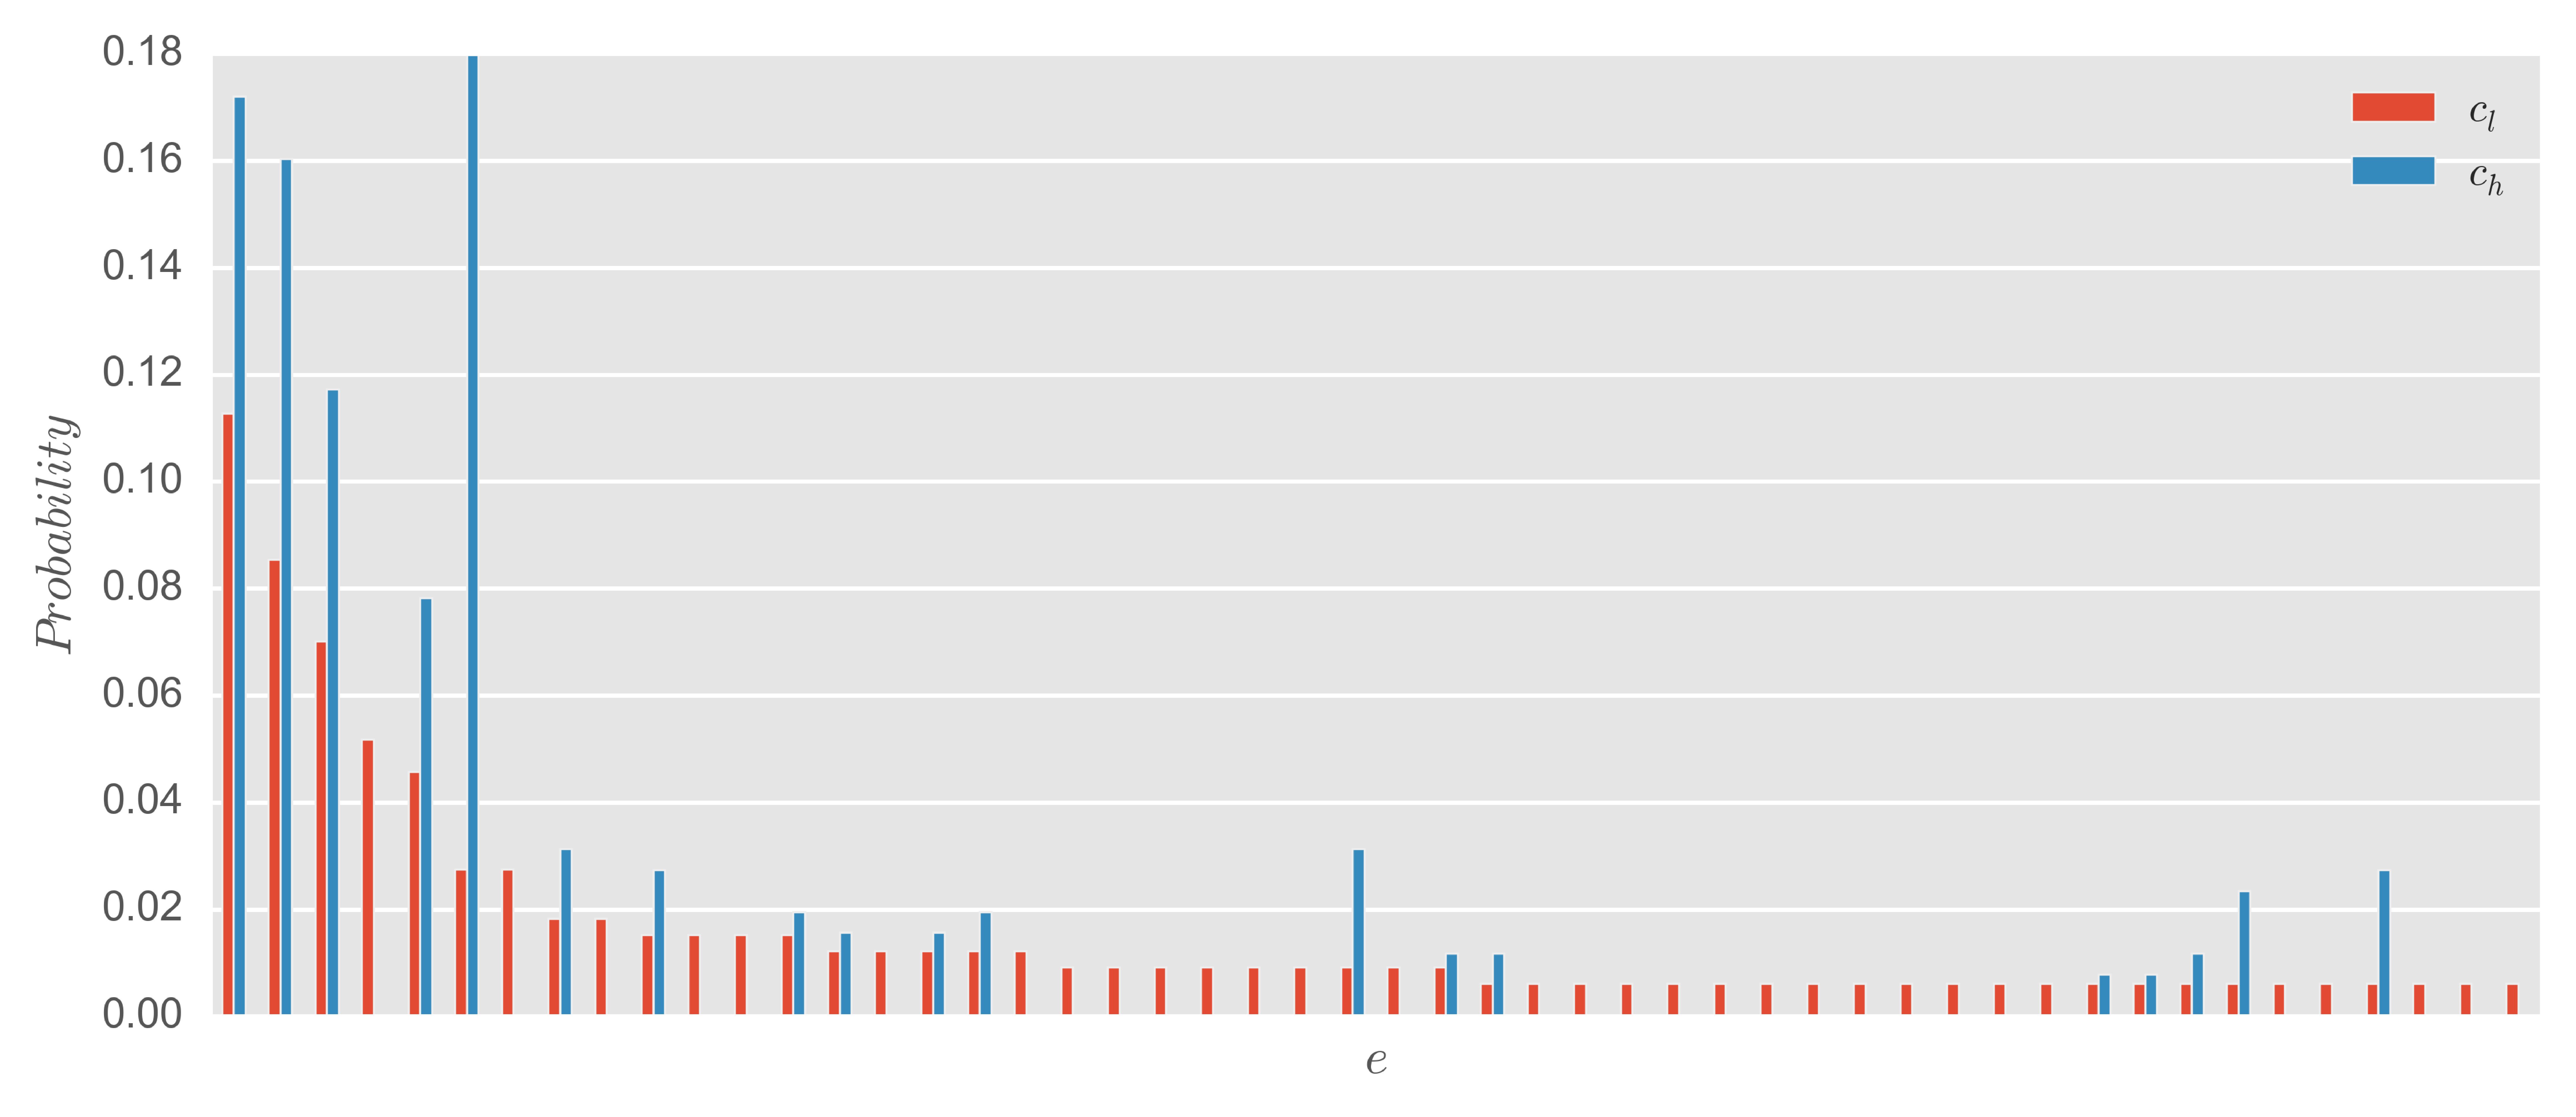
\epsfig{file=resources/df_hac_50_bill_gates.eps,width=\columnwidth, height=0.3\columnwidth}
\caption{Comparison between $P(h|e)$) and $\hat{P}(h|e)$ for \at{Bill Gates}. \small The red bars means $P(c|e)$ and the blue ones represents $\hat{P}(h|e)$. Only top 50 concepts are shown due to space limit.  }
\label{fig:hac}
\vspace{-6mm}
\end{figure}

\nop{
\xch{not really need to be similar with the original, but I will do it}. We report the Pearson correlation between....

We further give case studies in Table.~\ref{tab:rerank} with the comparison to the direct estimation of $P(c|e)$ using Probase. 
}
%
%\begin{table*}[htbp!]
%  \centering
%  \caption{Rerank comparation}
%    \begin{tabular}{llrrlrr}
%    \toprule
%    \multicolumn{1}{c}{} & \multicolumn{3}{c}{aggregated} & \multicolumn{3}{c}{original head concepts} \\
%    \midrule
%    \multicolumn{1}{c}{Entity} & agg head & agg count & agg prob & org head & org count & org prob \\
%    \midrule
%    \multicolumn{1}{c}{\multirow{10}[0]{*}{shanghai}} & city  & 1311  & 0.829222 & city  & 644   & 0.407337 \\
%    \multicolumn{1}{c}{} & region & 46    & 0.029096 & region & 27    & 0.017078 \\
%    \multicolumn{1}{c}{} & area  & 42    & 0.026565 & metropolis & 23    & 0.014548 \\
%    \multicolumn{1}{c}{} & metropolis & 26    & 0.016445 & megacities & 15    & 0.009488 \\
%    \multicolumn{1}{c}{} & port  & 20    & 0.01265 & market & 15    & 0.009488 \\
%    \multicolumn{1}{c}{} & market & 19    & 0.012018 & location & 15    & 0.009488 \\
%    \multicolumn{1}{c}{} & centre & 18    & 0.011385 & port  & 9     & 0.005693 \\
%    \multicolumn{1}{c}{} & location & 17    & 0.010753 & locality & 6     & 0.003795 \\
%    \multicolumn{1}{c}{} & megacities & 15    & 0.009488 & locale & 5     & 0.003163 \\
%    \multicolumn{1}{c}{} & center & 11    & 0.006958 & seaport & 4     & 0.00253 \\
%          &       &       &       &       &       &  \\
%    \multicolumn{1}{c}{\multirow{10}[0]{*}{bill gates}} & leader & 46    & 0.140244 & billionaire & 37    & 0.112805 \\
%    \multicolumn{1}{c}{} & billionaire & 44    & 0.134146 & entrepreneur & 28    & 0.085366 \\
%    \multicolumn{1}{c}{} & entrepreneur & 41    & 0.125 & philanthropist & 23    & 0.070122 \\
%    \multicolumn{1}{c}{} & philanthropist & 30    & 0.091463 & celebrity & 15    & 0.045732 \\
%    \multicolumn{1}{c}{} & celebrity & 20    & 0.060976 & leader & 9     & 0.027439 \\
%    \multicolumn{1}{c}{} & person & 16    & 0.04878 & innovator & 6     & 0.018293 \\
%    \multicolumn{1}{c}{} & figure & 11    & 0.033537 & personality & 5     & 0.015244 \\
%    \multicolumn{1}{c}{} & innovator & 8     & 0.02439 & expert & 5     & 0.015244 \\
%    \multicolumn{1}{c}{} & luminary & 8     & 0.02439 & folks & 4     & 0.012195 \\
%    \multicolumn{1}{c}{} & individual & 7     & 0.021341 & icon  & 4     & 0.012195 \\
%          &       &       &       &       &       &  \\
%    \multicolumn{1}{c}{\multirow{10}[0]{*}{samsung}} & company & 1030  & 0.376875 & company & 816   & 0.298573 \\
%    \multicolumn{1}{c}{} & brand & 829   & 0.30333 & brand & 561   & 0.205269 \\
%    \multicolumn{1}{c}{} & manufacturer & 238   & 0.087084 & client & 42    & 0.015368 \\
%    \multicolumn{1}{c}{} & maker & 112   & 0.040981 & firm  & 39    & 0.01427 \\
%    \multicolumn{1}{c}{} & player & 60    & 0.021954 & rival & 38    & 0.013904 \\
%    \multicolumn{1}{c}{} & phone & 60    & 0.021954 & player & 33    & 0.012075 \\
%    \multicolumn{1}{c}{} & giant & 51    & 0.018661 & phone & 30    & 0.010977 \\
%    \multicolumn{1}{c}{} & firm  & 49    & 0.017929 & conglomerate & 19    & 0.006952 \\
%    \multicolumn{1}{c}{} & name  & 49    & 0.017929 & corporation & 19    & 0.006952 \\
%    \multicolumn{1}{c}{} & conglomerate & 42    & 0.015368 & partner & 12    & 0.004391 \\
%          &       &       &       &       &       &  \\
%    \multicolumn{1}{c}{\multirow{10}[0]{*}{mona lisa}} & painting & 56    & 0.4   & painting & 33    & 0.235714 \\
%    \multicolumn{1}{c}{} & masterpiece & 21    & 0.15  & masterpiece & 16    & 0.114286 \\
%    \multicolumn{1}{c}{} & work  & 20    & 0.142857 & work  & 10    & 0.071429 \\
%    \multicolumn{1}{c}{} & film  & 6     & 0.042857 & film  & 5     & 0.035714 \\
%    \multicolumn{1}{c}{} & image & 5     & 0.035714 & image & 3     & 0.021429 \\
%    \multicolumn{1}{c}{} & artwork & 4     & 0.028571 & picture & 3     & 0.021429 \\
%    \multicolumn{1}{c}{} & portrait & 4     & 0.028571 & treasure & 2     & 0.014286 \\
%    \multicolumn{1}{c}{} & piece & 4     & 0.028571 & song  & 2     & 0.014286 \\
%    \multicolumn{1}{c}{} & picture & 3     & 0.021429 & icon  & 2     & 0.014286 \\
%    \multicolumn{1}{c}{} & figure & 3     & 0.021429 & artwork & 1     & 0.007143 \\
%    \bottomrule
%
%    \end{tabular}%
%  \label{tab:rerank}%
%\end{table*}%



%\subsection{Find alias}

%\subsubsection{compare}
%
%In this section we compare $ P(<c_1,c_2 >|a )$ with $ P(c_1|a) \times P(c_2|a)$ to show that

\subsection{Exp 3: Joint Conceptualization}
Now, we evaluate the effectiveness of joint conceptualization, which is implemented by the introduction of $\alpha(c_1,c_2)$ in Eq.~\ref{eq:target_expand2_jr}. 
We compare to the baseline method in Eq~\ref{eq:naive}.
We present Table~\ref{tab:expjc} to show many cases where $\alpha$ help identify the true concept pair (ranked as the first).
To see the effectiveness of our approach, we arbitrarily select entities with multiple senses as $e_1$. 
From the results, we can see that (1) the result with $\alpha$ is significantly better and (2) joint conceptualization in general can resolve the ambiguity of entities. For instance, \at{apple} isA \at{fruit} given a pair \at{<apple, steve jobs>}.

\begin{table}[htbp]
  \vspace{-6mm}
  \centering
  \caption{Joint Conceptualization with and without $\alpha$}
    \begin{tabular}{rrrr}
    \toprule
    $e_1$                               & $e_2$                               & $c_1 $  without $\alpha$       & $c_1$  with $\alpha$ \\
    \midrule
    columbia                            & barack obama                        & country                    & \textbf{school }\\
    apple                               & steve jobs                          & fruit                & \textbf{company} \\
   da vinci code           & ron howard                       & book                     & \textbf{film} \\
    spa                                 & belgium                             & facility                  & \textbf{place} \\
    \bottomrule
    \end{tabular}%
  \label{tab:expjc}%
  
  \vspace{-6mm}
\end{table}%



%
%{\bf Since there are many entities belongs to the same concept and we only consider topK $(c_1,c_2)$ pairs that has high typicality $P( (c_1,c_2) |a)$, so that the weird $(c_1,c_2)$ patterns as manifest in Example.~\ref{exa:sd} can be easily filtered.}
%
%\begin{figure}[!htb]
%\centering 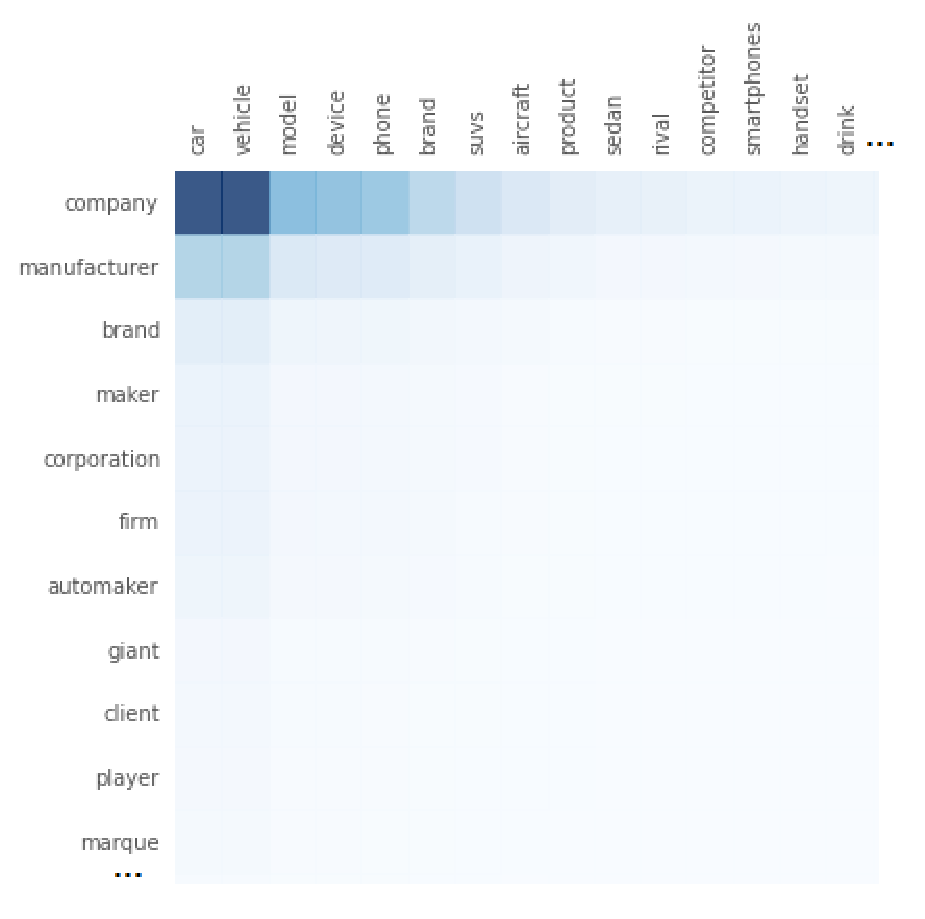
\epsfig{file=resources/ev_plot_manufacturer.eps,width=2.5in}
%\caption{$(c_1,c_2$) plot for attribute \term{Manufacturer}. } \label{fig:evplot}
%\end{figure}
%
%\begin{example}[Sense Disambiguation]
%Consider the following $(e1,a,e2)$ tuple \term{(iphone, manufacturer, apple)}. Suppose it is our query, where \term{apple}'s sense can either be a kind of \term{fruit} or a \term{company}.
%Fig.~\ref{fig:evplot} is a heatmap for all the concepts pairs $(c_1,c_2)$ of attributes \term{manufacturer}. The horizontal axis represents the $e_1$ and the vertical axis stands for $e_2$. The darker the blue is, the higher typicality it will be. In Fig.~\ref{fig:evplot}, We can observe that the top concepts of $e_2$ in the heatmap are \term{company, manufacturer,...} and top 10 pairs also does not include \term{fruit}. The intuition for this is that there exists thousands of $(e1,a,e2)$ tuple such as \term{(BMW\_Z4,manufacturer,BMW),(PlayStation\_4,manufacturer,Sony)} other than \term{(iphone, manufacturer, apple)} tuple, which results in a reasonable distribution.
%\label{exa:sd}
%\end{example}
%
%We further present a comparison of Eq.~\ref{eq:target_expand2_jr} and Eq.~\ref{eq:target_expand2_naive}, where the conceptualization is done with and without multiplying $\alpha(c_1,c_2)$.
%
%\begin{figure}[!htb]
%\centering
%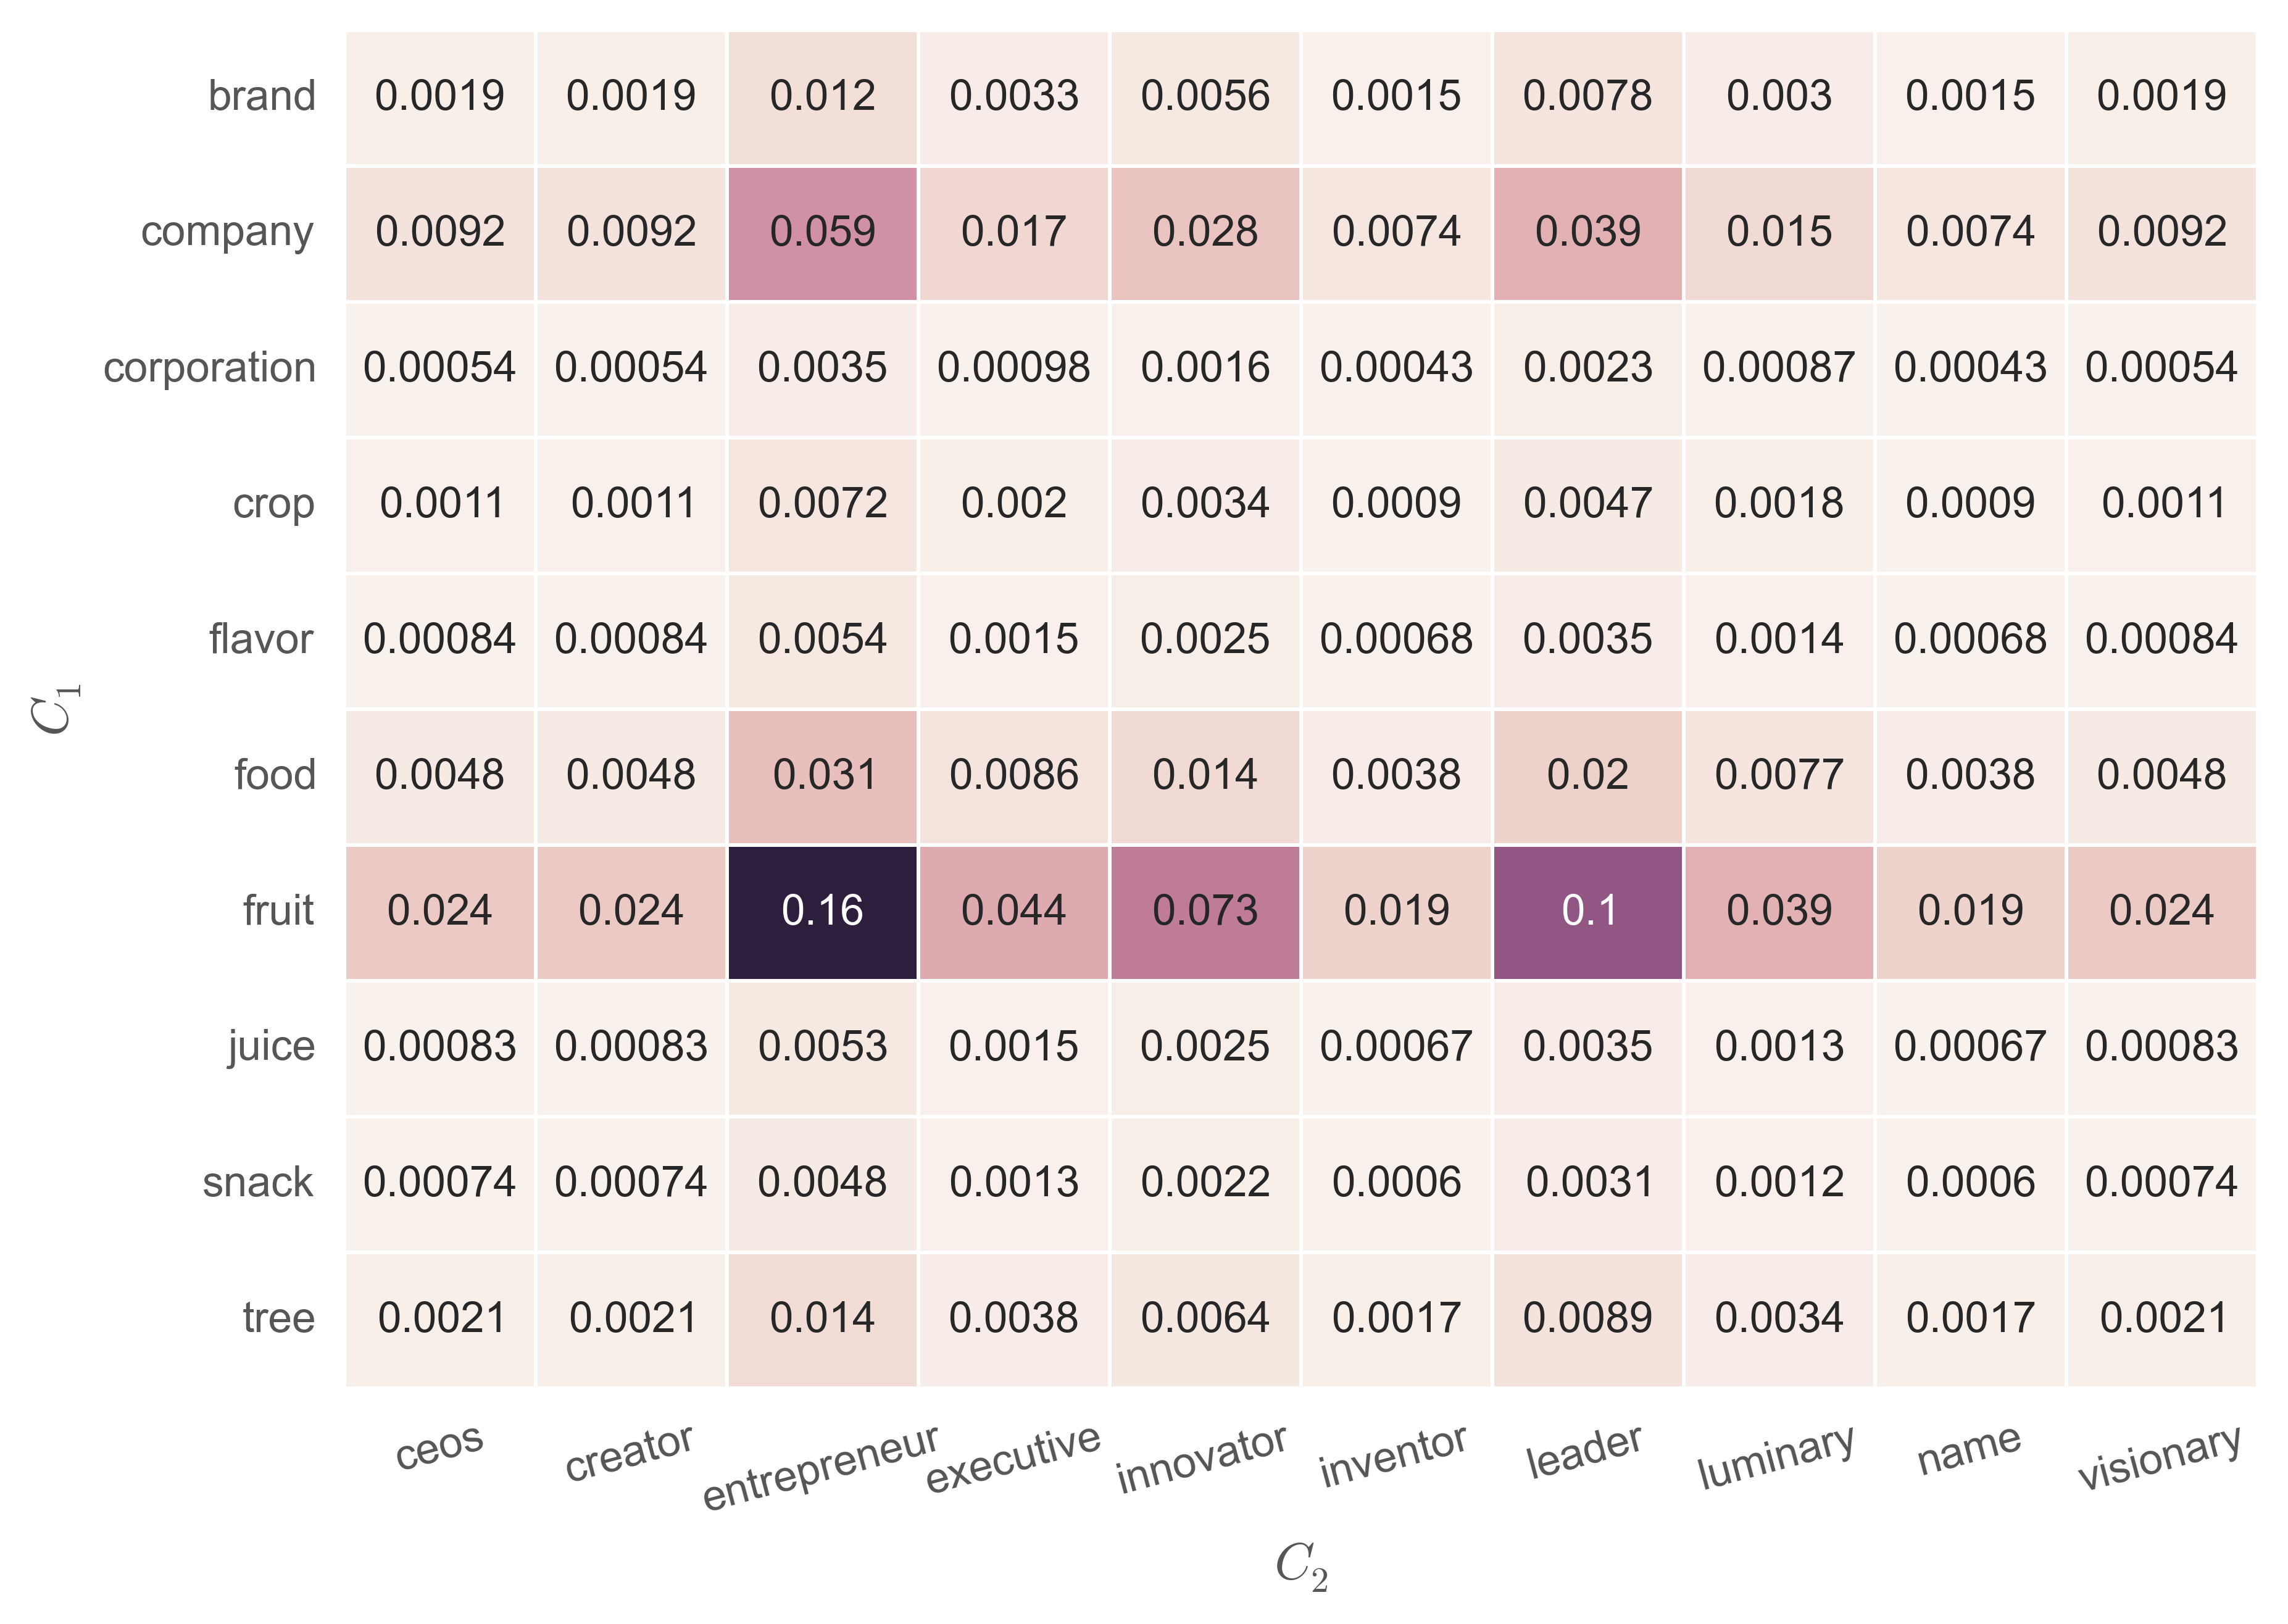
\epsfig{file=resources/df_for_plot_foundedBy.eps,width=\columnwidth }
%\caption{Distribution of $P(\langle c_1,c_2 \rangle|\langle e_1,e_2 \rangle )$ of attribute \at{foundedBy} \textbf{without} $\alpha$. }
%\label{fig:c1c2}
%\end{figure}
%
%\begin{figure}[!htb]
%\centering
%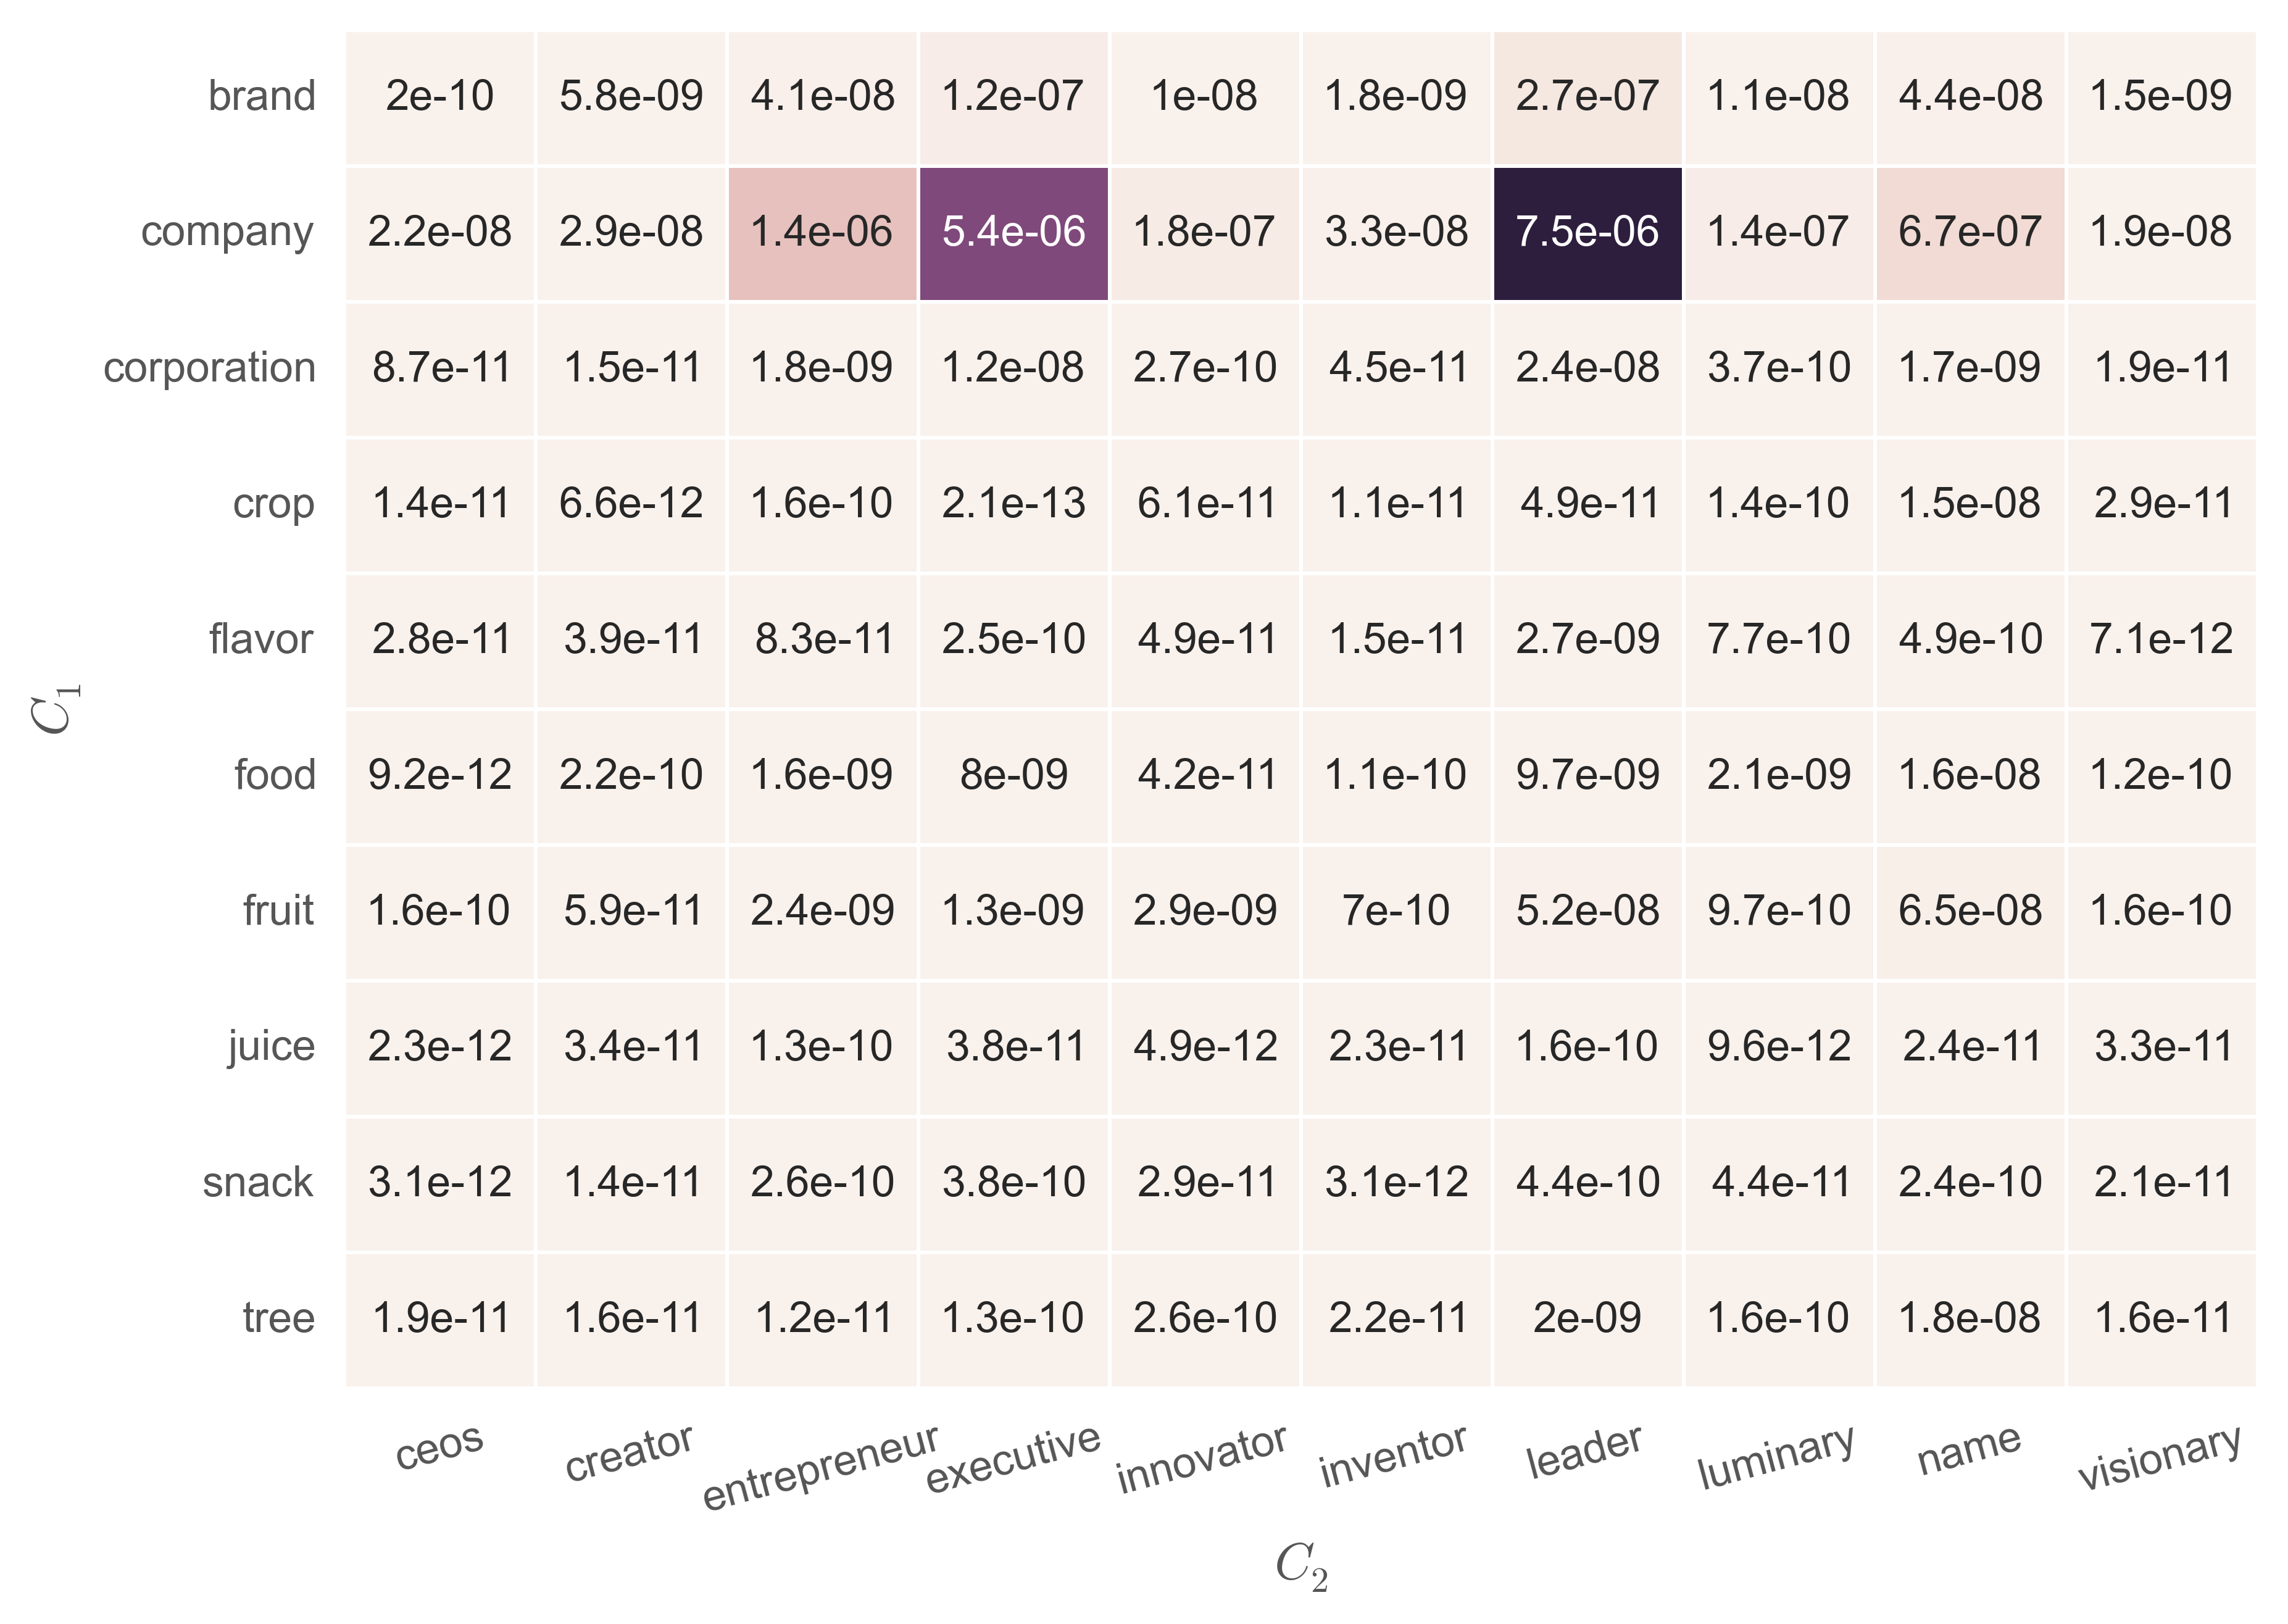
\epsfig{file=resources/df_for_plot_foundedBy_with_alpha_c1c2.eps,width=\columnwidth}
%\caption{Distribution of $P(\langle c_1,c_2 \rangle|\langle e_1,e_2 \rangle )$ of attribute \at{foundedBy} \textbf{with} $\alpha=P(\langle c_1,c_2 \rangle)$. }
%\label{fig:c1c2_alpha}
%\end{figure}
%
%\begin{figure}[!htb]
%\centering
%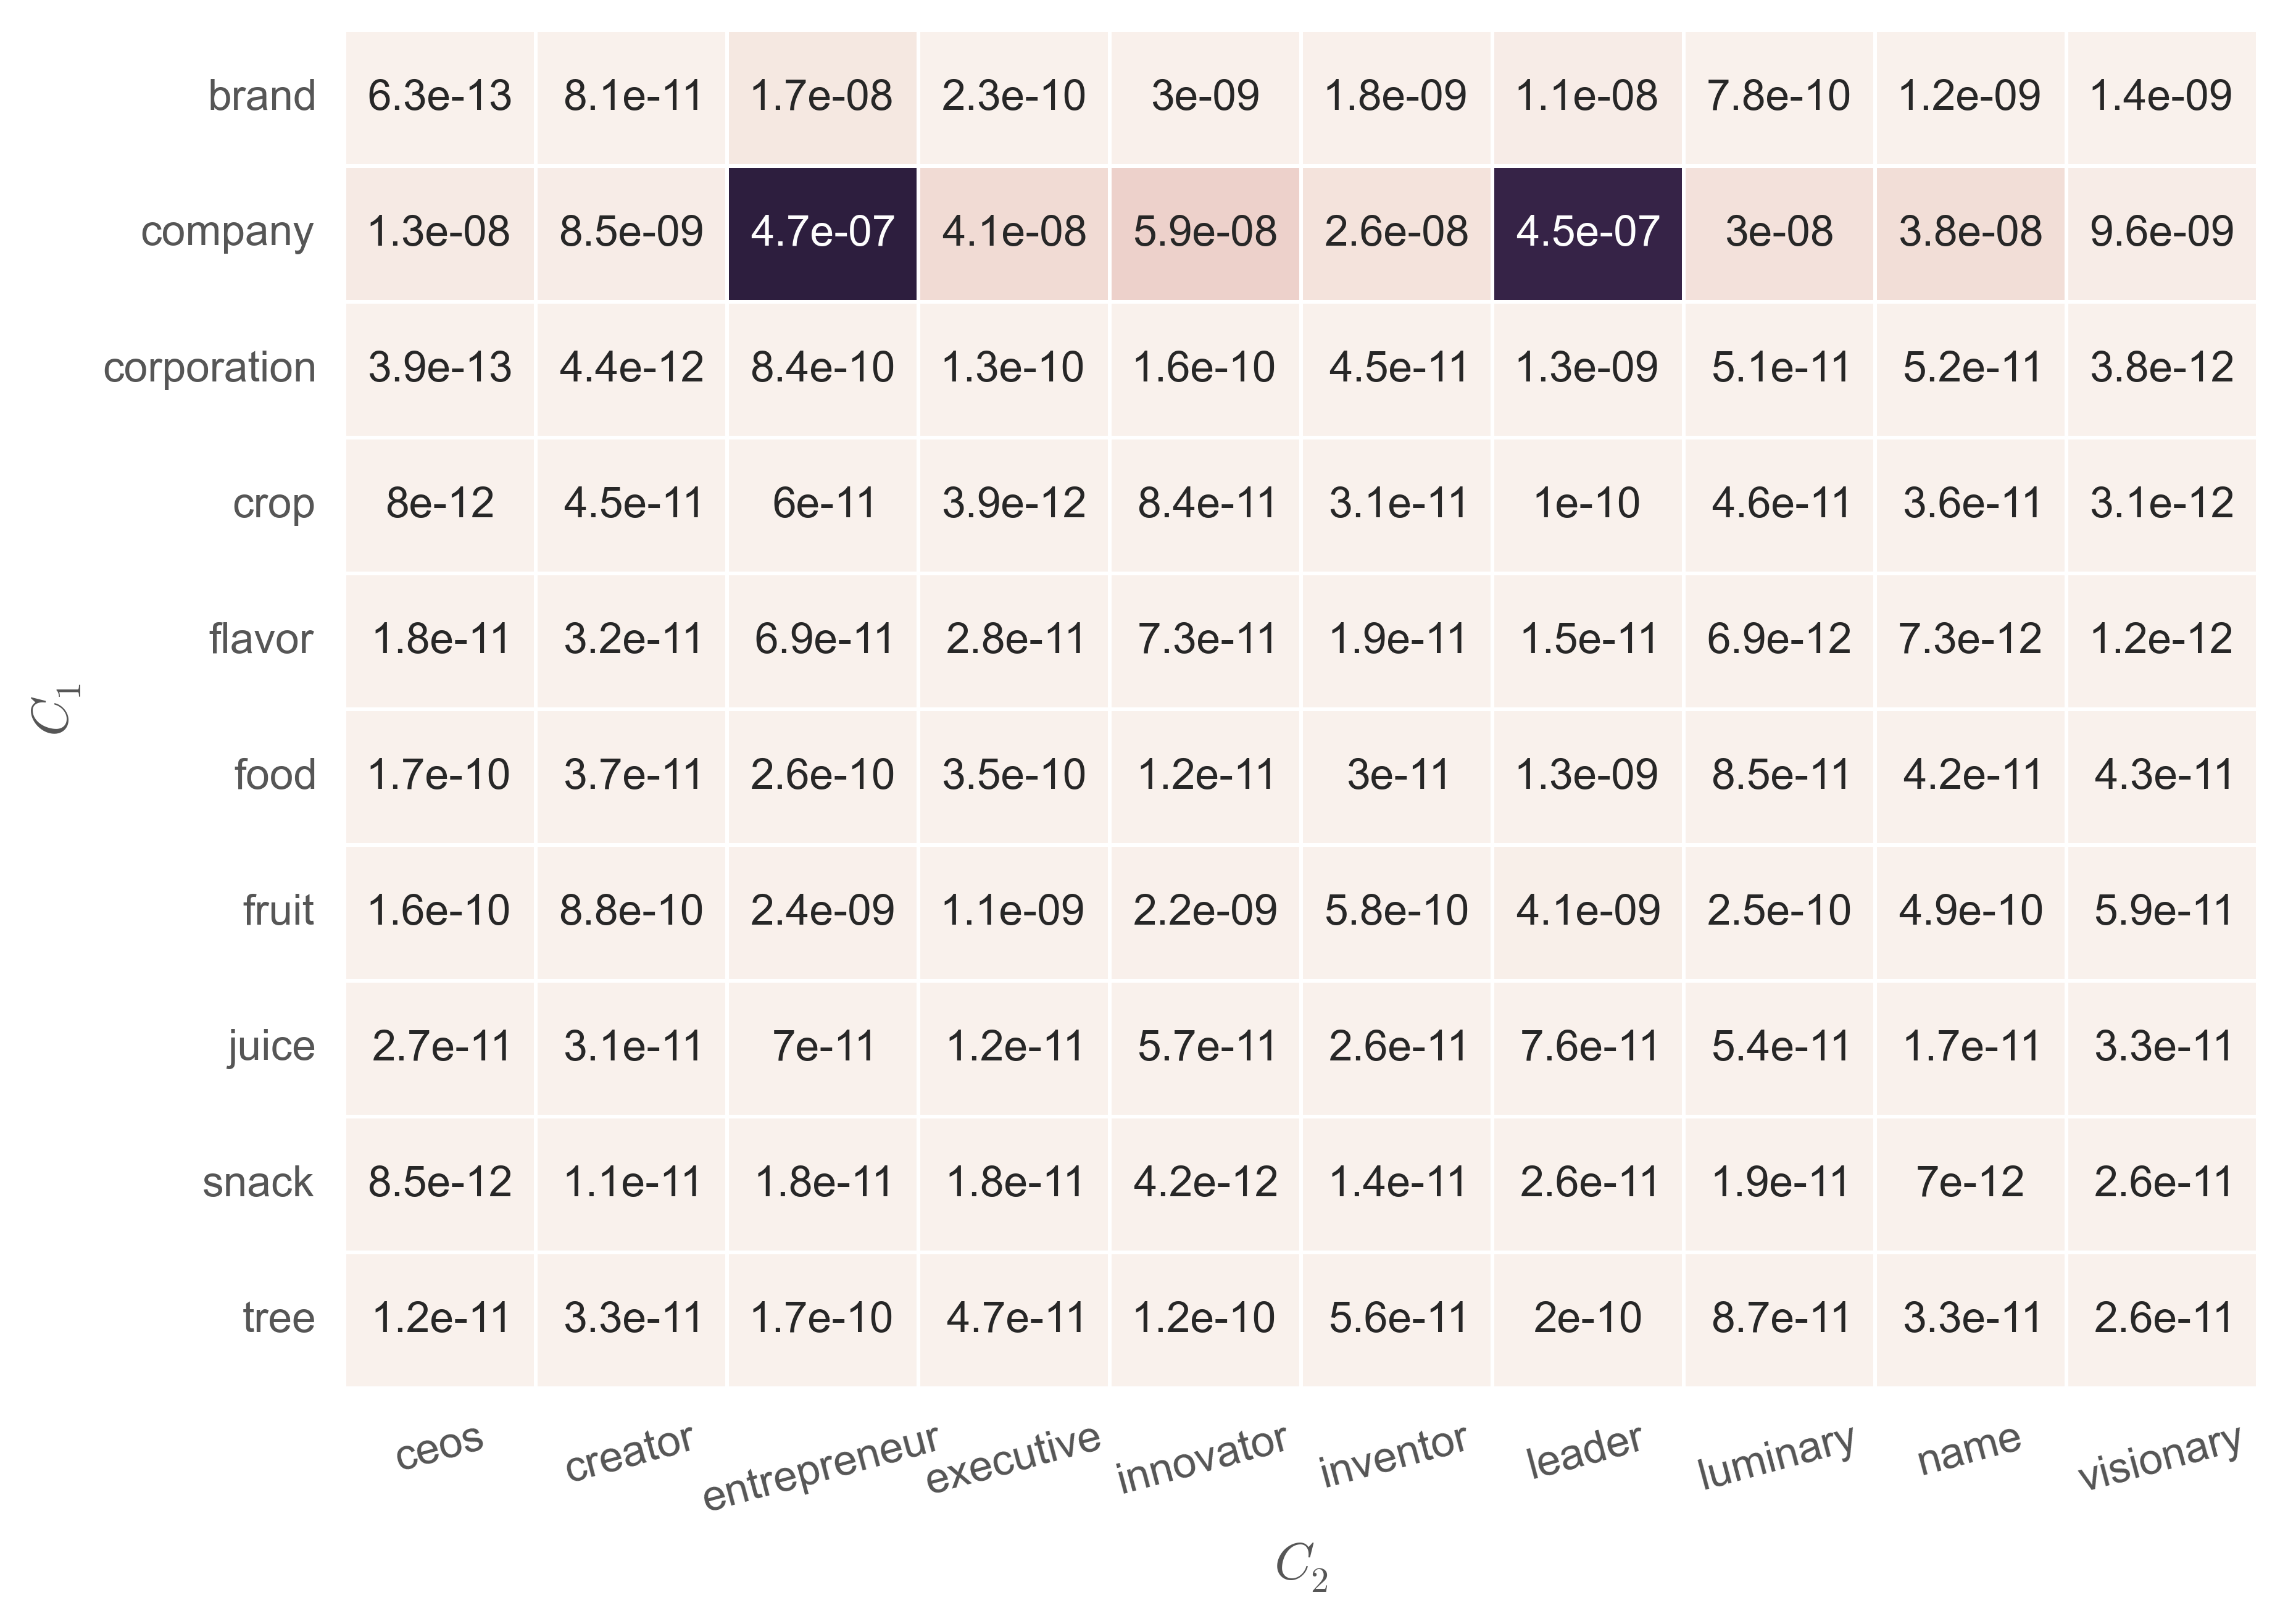
\epsfig{file=resources/df_for_plot_foundedBy_with_alpha.eps,width=\columnwidth}
%\caption{Distribution of $P(\langle c_1,c_2 \rangle|\langle e_1,e_2 \rangle )$ of attribute \at{foundedBy} \textbf{with} $\alpha=P(\langle c_1,c_2 \rangle|a)$. }
%\label{fig:c1c2_alpha_given_a}
%\end{figure}
%
%
%We present the visualization of the distribution of $P(\langle c_1,c_2 \rangle|\langle e_1,e_2 \rangle )$ for Eq.~\ref{eq:naive} in Figure~\ref{fig:c1c2} and for Eq.~\ref{eq:target_expand2_jr} in Figure~\ref{fig:c1c2_alpha}.
%The floats inside each box represents $P(\langle c_1,c_2 \rangle|\langle e_1,e_2 \rangle )$, when the pair $\langle c_1,c_2 \rangle$ does not exist, we add a small value to $\alpha$ and then do normalization for smoothing purpose.


\subsection{Exp 4: Collective Conceptualization}
We compare our approach with an $MDL$ based collective conceptualization solution~\cite{sunconceptual}, which aims at generating a minimum set of conceptual labels that best summarize a bag of words.
In our case, the bag of words are replaced by a set of entities.
$MDL$ uses $\alpha$ to tune the balance between \ac{Minimality} and \ac{Coverage}. 
Bigger $\alpha$ lead to better coverage as well as general concepts.
We set the parameter $\alpha$ in $MDL$ to 0.5 for normal comparison and 0.1 for gaining more concept pairs.

In the experiment, we select 50 attributes from different relation groups (such as \ac{PERSON-ORGNIZATION, PERSON-AFFLIATION, OBJECT-LOCATION} etc.\ ) and manually evaluate the top 20 concept pairs for each attribute.
Volunteers give a score \textbf{2} for excellent concept pairs (e.g. \at{<company, entrepreneur>} for \at{FoundedBy}), \textbf{1} for correct while not appropriate ones (e.g. \at{<song, celebrity>} for \at{writer} ), and \textbf{0} for wrong concept pairs (e.g. \at{<topic, Country>} for \at{SpokenIn}).
We present the human evaluated score in Figure~\ref{fig:eva_violin_pc1c2ga}.
We also show the evaluation results on each relation relation group produced by $ERF$ in Figure~\ref{fig:eva_violin_group}.

\begin{figure}[!htb]
\centering
\footnotesize
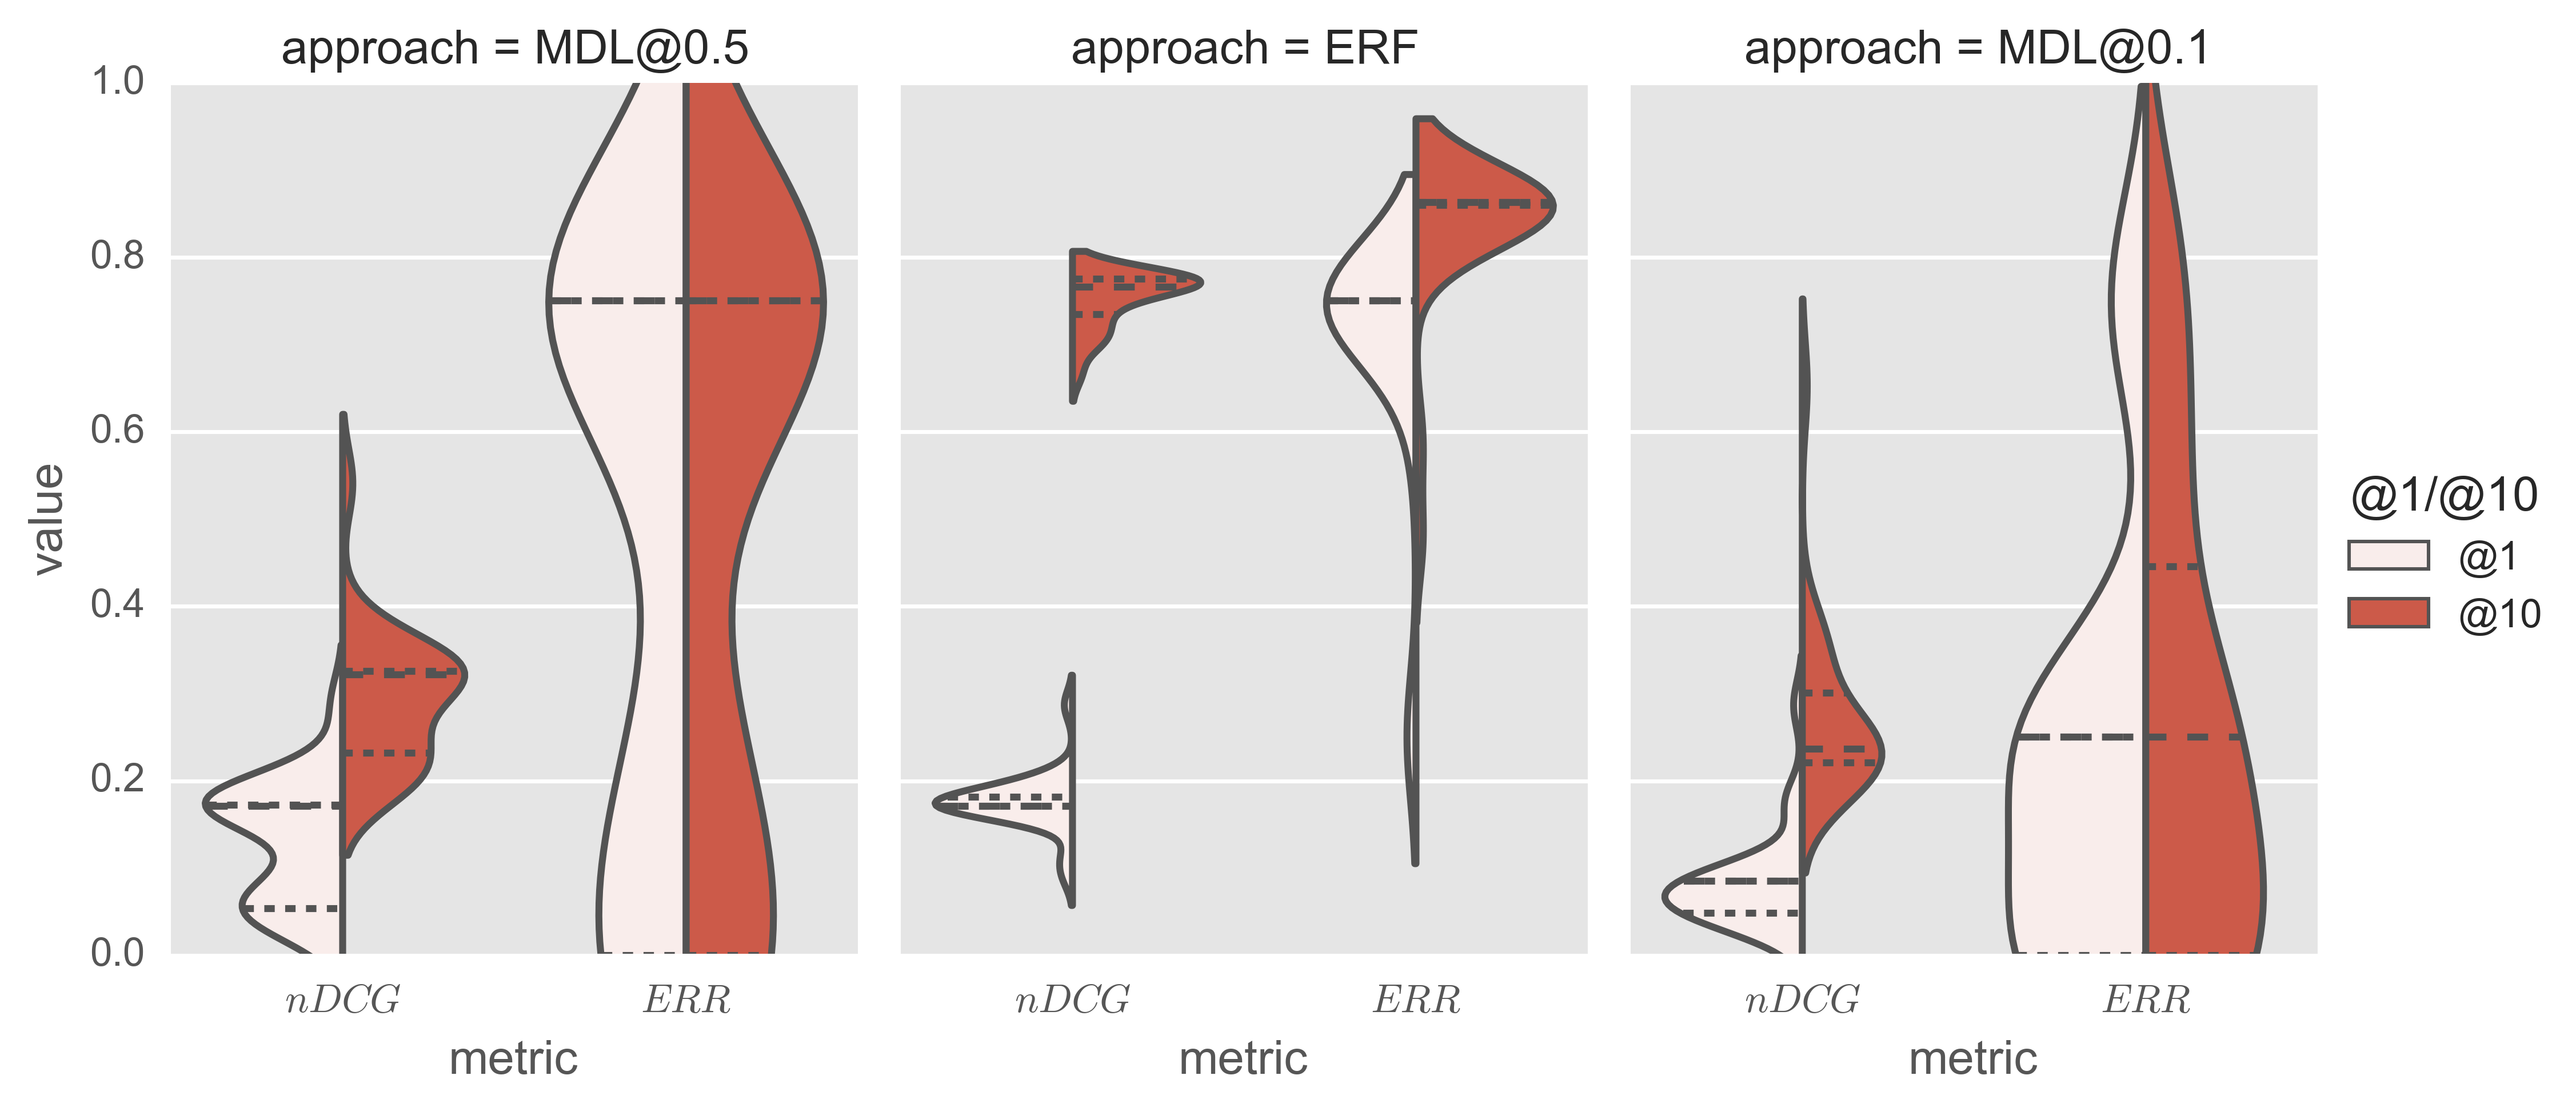
\epsfig{file=resources/violin_eval.eps,width=1.1\columnwidth}
\vspace{-7mm}
\caption{\small Distribution of human evaluation result for $P(\langle c_1,c_2 \rangle|a)$. \footnotesize The white part is metric@1 and the red part is metric@10. Dashed line means quartiles of the distribution. The $ERF$ in the middle is our result, compared with $MDL@\alpha=0.5$ (left) and $MDL@\alpha=0.1$(right). }
\label{fig:eva_violin_pc1c2ga}
\vspace{-4mm}
\end{figure}

From the results we can see that $ERF$ always produces the best result in terms of $nDCG@1$ and $nDCG@10$.
We can observe a significant increase in the $nDCG@10$ score for $ERF$ while not much increase in $MDL$-based approach. Because $MDL$ tends to give as few concepts as possible and sacrifices the coverage when $\alpha$ is small. The $nDCG@1$ score is reasonably low since usually there are more than one pair of correct concepts.

%All these results can be consistently observed across different relationships as seen in Figure~\ref{fig:eva_violin_group}.

The $ERR@1$ and $ERR@10$ measure vary not that much due to its user-behavioral instinct. In general, a real user pays less attention to the lower-ranked pairs after he/she find the correct concept pair.
The results show that 
 $ERF$ always performs best and gains an slight increase in $ERR@10$ compared to $ERR@1$.
 The results are consistent across different groups of relationships.

%\begin{figure*}[!htb]
%\centering
%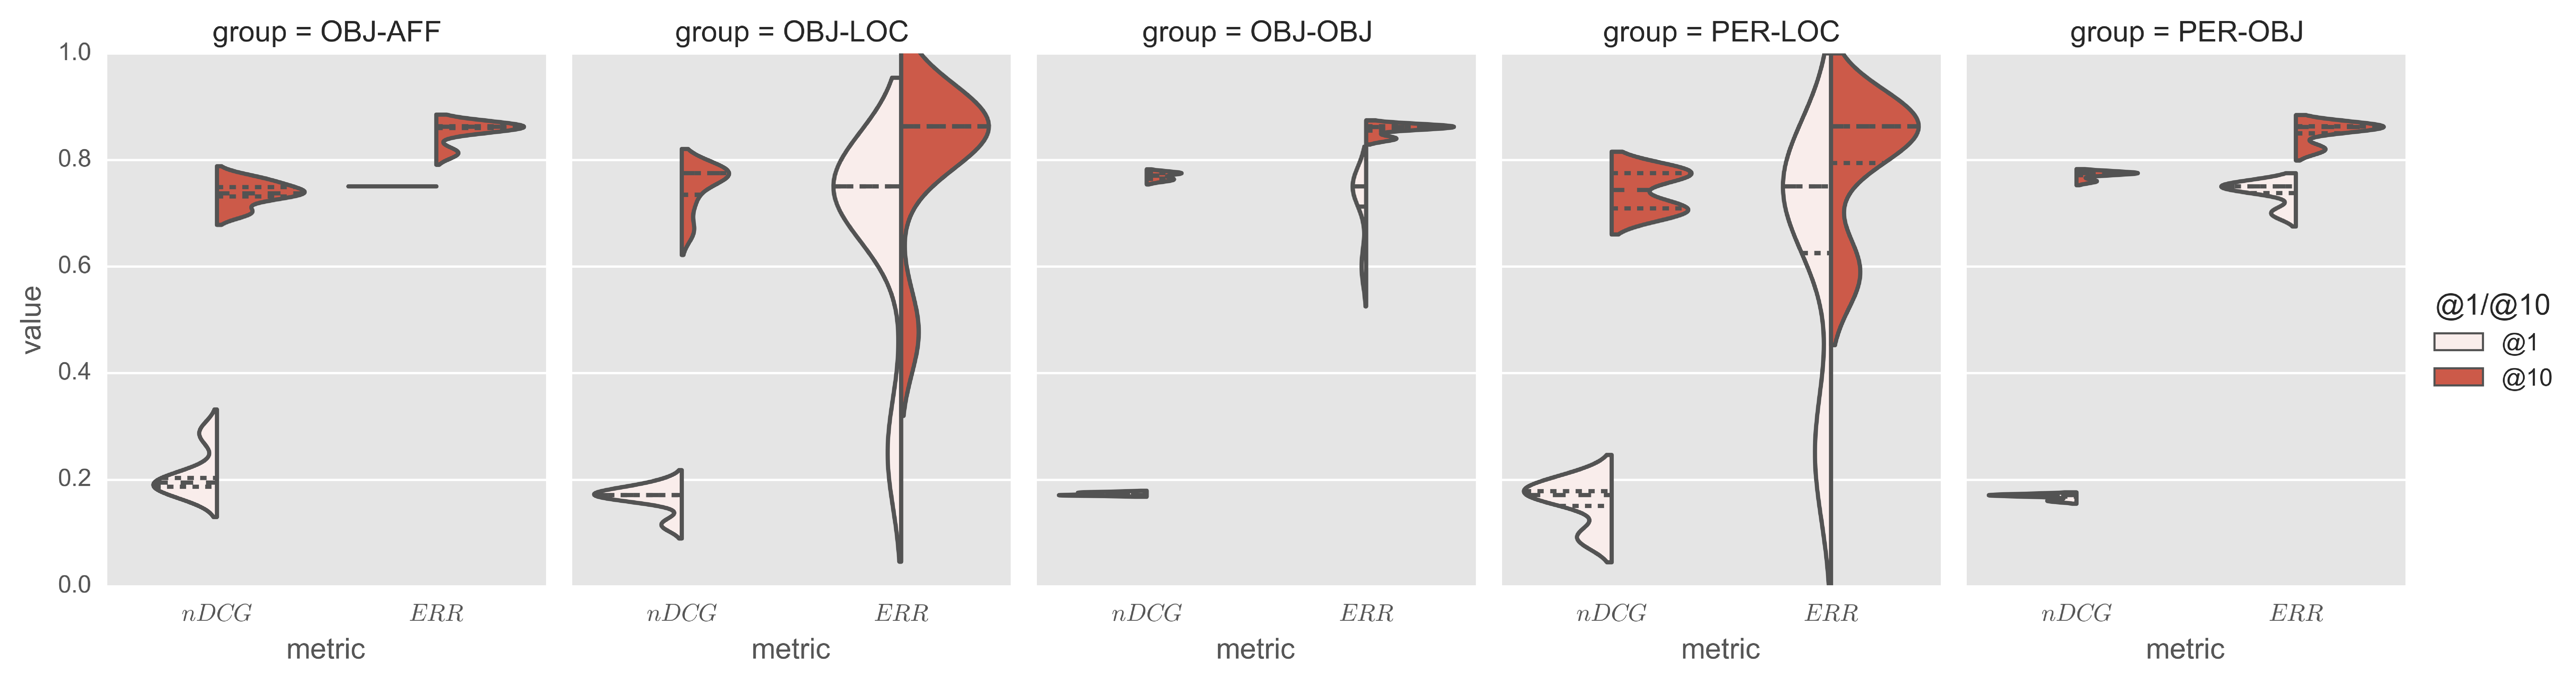
\epsfig{file=resources/violin_eval_group.eps,width=2.2\columnwidth}
%\caption{Distribution of human evaluation result for $P(\langle c_1,c_2 \rangle|a)$ produced by $ERF$. \small Each seperate graph represents a certain relation group.}
%\label{fig:eva_violin_group}
%\vspace{-6mm}
%\end{figure*}



\subsection{Case Study}

We show some of the relations that has been retrieved by our method in Table~\ref{tab:results}.
The first 2 columns show the query entity pair.
The 3rd column is the relation retrieved by $ERF$ with a confidence score in the 4th column.
Note that we combine the relationships of $\langle e_1,e_2\rangle$ and $\langle e_2,e_1\rangle$ together.
For example the relation \at{commander} of \at{<adolf hitler,world war ii>} is actually the attribute of \at{<world war ii, adolf hilter>}. From the table, we can see that most top one relation is the right attribute between the entity pair.
For some entity pairs, the top 2 or 3 relations are also reasonable, for example the \at{<apple, steve jobs>} case.
All these case studies sufficiently show the effectiveness of ERF.
% Table generated by Excel2LaTeX from sheet 'Sheet1'
\begin{table}[ht!]
\vspace{-6mm}
  \centering
  \caption{First three results produced by ERF}
  \small
    \begin{tabular}{cccr}
    \toprule
    Entity1 & Entity2 & Relation & Score ($\times10^{-3}$) \\
    \midrule
    \multicolumn{1}{c}{\multirow{3}{*}{\parbox{1cm}{ Sherlock Holmes}}} & \multicolumn{1}{c}{\multirow{3}[0]{*}{united kingdom}} & anthem & 7.0 \\
    \multicolumn{1}{c}{} & \multicolumn{1}{c}{} & firstAppearance & 4.5 \\
    \multicolumn{1}{c}{} & \multicolumn{1}{c}{} & allegiance & 4.4 \\
    \hline
    \multicolumn{1}{c}{\multirow{3}{*}{\parbox{1cm}{\centering apple}}} & \multicolumn{1}{c}{\multirow{3}[0]{*}{steve jobs}} & foundedBy & 0.015439 \\
    \multicolumn{1}{c}{} & \multicolumn{1}{c}{} & keyPerson & 0.009932 \\
    \multicolumn{1}{c}{} & \multicolumn{1}{c}{} & successor & 0.008069 \\
    \hline
    \multicolumn{1}{c}{\multirow{3}{*}{\parbox{1cm}{\centering Adolf Hitler}}} & \multicolumn{1}{c}{\multirow{3}[0]{*}{world war ii}} & commander & 0.037712 \\
    \multicolumn{1}{c}{} & \multicolumn{1}{c}{} & battle & 0.022161 \\
    \multicolumn{1}{c}{} & \multicolumn{1}{c}{} & ceo   & 2.44E-05 \\
    \hline
    \multicolumn{1}{c}{\multirow{3}{*}{\parbox{1cm}{\centering Microsoft}}} & \multicolumn{1}{c}{\multirow{3}[0]{*}{redmond}} & locationCity & 0.082507 \\
    \multicolumn{1}{c}{} & \multicolumn{1}{c}{} & foundationPlace & 0.047192 \\
    \multicolumn{1}{c}{} & \multicolumn{1}{c}{} & location & 0.036916 \\
    \hline
    \multicolumn{1}{c}{\multirow{3}{*}{Titanic}} & \multicolumn{1}{c}{\multirow{3}[0]{*}{James Cameron}} & director & 0.124407 \\
    \multicolumn{1}{c}{} & \multicolumn{1}{c}{} & cinematography & 0.096447 \\
    \multicolumn{1}{c}{} & \multicolumn{1}{c}{} & editing & 0.080134 \\
    \hline
    \multicolumn{1}{c}{\multirow{3}{*}{Titanic}} & \multicolumn{1}{c}{\multirow{3}[0]{*}{Leonardo Dicaprio}} & starring & 0.049689 \\
    \multicolumn{1}{c}{} & \multicolumn{1}{c}{} & narrator & 0.037267 \\
    \multicolumn{1}{c}{} & \multicolumn{1}{c}{} & producer & 0.01306 \\
    \hline
    \multicolumn{1}{c}{\multirow{3}{*}{\parbox{1cm}{\centering Harry Potter}}} & \multicolumn{1}{c}{\multirow{3}[0]{*}{J K rowling}} & notableWork & 0.016965 \\
    \multicolumn{1}{c}{} & \multicolumn{1}{c}{} & author & 0.015514 \\
    \multicolumn{1}{c}{} & \multicolumn{1}{c}{} & coverArtist & 0.014906 \\
    \bottomrule
    \end{tabular}%
  \label{tab:results}%
\end{table}%


%\subsection{Selectional Preference}

\vspace{-2mm}
\section{Conclusion}
\label{sec:conclusion}

We studied the problem of explaining the relationship between two Wikipedia pages that are hyperlinked. If there exists a SPO triple explicitly explaining the relationship, this problem degenerates to the retrieval of such triple. However, we found such case is extremely rare, 1.5\%, and thus increasing recall for the rest pairs is crucial. We proposed to use concept pairs as intermediate variables to find a typical attribute for this pair as a possible explanation. We observed that, to ensure accuracy, such conceptualization should jointly optimize for both entities and identify head concepts. We validated our framework using real-life Wikipedia entities and taxonomies.

\newpage	

\small
\bibliographystyle{aaai}
%\bibliographystyle{abbrv}
\bibliography{refer}

\end{document}
